%------------------------------------------------------------------------------
%
%  IgH EtherCAT Master Documentation
%
%  $Id$
%
%  vi: spell spelllang=en tw=78
% 
%------------------------------------------------------------------------------

\documentclass[a4paper,12pt,BCOR6mm,bibtotoc,idxtotoc]{scrbook}

\usepackage[latin1]{inputenc}
\usepackage[automark,headsepline]{scrpage2}
\usepackage{graphicx}
\usepackage{makeidx}
\usepackage[refpage]{nomencl}
\usepackage{listings}
\usepackage[nofancy]{rcsinfo}
\usepackage{SIunits}
\usepackage{amsmath} % for \text{}
\usepackage{hyperref}

\hypersetup{pdfpagelabels,plainpages=false}
\hypersetup{linkcolor=blue,colorlinks=true,urlcolor=blue}

\setlength{\parskip}{0.8ex plus 0.8ex minus 0.5ex}
\setlength{\parindent}{0mm}

\setcounter{secnumdepth}{\subsubsectionlevel}

\DeclareFontShape{OT1}{cmtt}{bx}{n}
{
  <5><6><7><8><9><10><10.95><12><14.4><17.28><20.74><24.88>cmttb10
}{}

\lstset{basicstyle=\ttfamily\small,numberstyle=\tiny,aboveskip=4mm,
  belowskip=2mm,escapechar=`}
\renewcommand\lstlistlistingname{List of Listings}

% Workaround for lstlistoflistings bug
\makeatletter% --> De-TeX-FAQ
\renewcommand*{\lstlistoflistings}{%
  \begingroup
    \if@twocolumn
      \@restonecoltrue\onecolumn
    \else
      \@restonecolfalse
    \fi
    \lol@heading
    \setlength{\parskip}{\z@}%
    \setlength{\parindent}{\z@}%
    \setlength{\parfillskip}{\z@ \@plus 1fil}%
    \@starttoc{lol}%
    \if@restonecol\twocolumn\fi
  \endgroup
}
\makeatother% --> \makeatletter

\renewcommand\nomname{Glossary}

\newcommand{\IgH}{\raisebox{-0.7667ex}
  {
\includegraphics[height=2.2ex]{images/ighsign}}}

\rcsInfo $RCSId$

\newcommand{\masterversion}{1.5.0}
\newcommand{\linenum}[1]{\normalfont\textcircled{\tiny #1}}

\makeindex
\makenomenclature

% Revision and date on inner footer
\ifoot[\scriptsize\rcsInfoRevision, \rcsInfoDate]
    {\scriptsize\rcsInfoRevision, \rcsInfoDate}

%------------------------------------------------------------------------------

\begin{document}

\pagenumbering{roman}
\pagestyle{empty}

\begin{titlepage}
  \begin{center}
    \rule{\textwidth}{1.5mm}

    {\Huge\sf\textbf{IgH 
\includegraphics[height=2.4ex]{images/ethercat}
      Master \masterversion}\\[1ex]
      \textbf{Documentation}}

    \vspace{1ex}
    \rule{\textwidth}{1.5mm}

    \vspace{\fill} {\Large Dipl.-Ing. (FH) Florian Pose,
    \url{fp@igh-essen.com}\\[1ex] Ingenieurgemeinschaft \IgH}

    \vspace{\fill}
    {\Large Essen, \rcsInfoLongDate\\[1ex]
      Revision \rcsInfoRevision}
  \end{center}
\end{titlepage}

%------------------------------------------------------------------------------

\pagestyle{scrplain}

\tableofcontents
\listoftables
\listoffigures
%\lstlistoflistings

%------------------------------------------------------------------------------

\newpage
\pagestyle{scrheadings}

\section*{Conventions}
\addcontentsline{toc}{section}{Conventions}
\markleft{Conventions}

The following typographic conventions are used:

\begin{itemize}

\item \textit{Italic face} is used for newly introduced terms and file names.

\item \texttt{Typewriter face} is used for code examples and command line
output.

\item \texttt{\textbf{Bold typewriter face}} is used for user input in command
lines.

\end{itemize}

Data values and addresses are usually specified as hexadecimal values. These
are marked in the \textit{C} programming language style with the prefix
\lstinline+0x+ (example: \lstinline+0x88A4+). Unless otherwise noted, address
values are specified as byte addresses.

Function names are always printed with parentheses, but without
parameters. So, if a function \lstinline+ecrt_request_master()+ has
empty parentheses, this shall not imply that it has no parameters.

If shell commands have to be entered, this is marked by a dollar prompt:

\begin{lstlisting}
$
\end{lstlisting}

Further, if a shell command has to be entered as the superuser, the
prompt is a mesh:

\begin{lstlisting}
#
\end{lstlisting}

%------------------------------------------------------------------------------

\chapter{The IgH EtherCAT Master}
\label{chapter:master}
\pagenumbering{arabic}

This chapter covers some general information about the EtherCAT master.

%------------------------------------------------------------------------------

\section{Feature Summary}
\label{sec:summary}
\index{Master!Features}

The list below gives a short summary of the master features.

\begin{itemize}

\item Designed as a kernel module for Linux 2.6.

\item Implemented according to IEC 61158-12 \cite{dlspec} \cite{alspec}.

\item Comes with EtherCAT-capable native drivers for several common Ethernet
chips, as well as a generic driver for all chips supported by the Linux
kernel.

  \begin{itemize}

  \item The native drivers operate the hardware without interrupts.

  \item Native drivers for additional Ethernet hardware can easily be
  implemented using the common device interface (see sec.~\ref{sec:ecdev})
  provided by the master module.

  \item For any other hardware, the generic driver can be used. It uses the
  lower layers of the Linux network stack.

  \end{itemize}

\item The master module supports multiple EtherCAT masters running in
parallel.

\item The master code supports any Linux realtime extension through its
independent architecture.

  \begin{itemize}

  \item RTAI\nomenclature{RTAI}{Realtime Application Interface} \cite{rtai},
  ADEOS\nomenclature{ADEOS}{Adaptive Domain Environment for Operating
  Systems}, RT-Preempt \cite{rt-preempt}, etc.

  \item It runs well even without realtime extensions.

  \end{itemize}

\item Common ``Application Interface'' for applications, that want to use
EtherCAT functionality (see chap.~\ref{chap:api}).

\item \textit{Domains} are introduced, to allow grouping of process
  data transfers with different slave groups and task periods.

  \begin{itemize}

  \item Handling of multiple domains with different task periods.

  \item Automatic calculation of process data mapping, FMMU and sync manager
  configuration within each domain.

  \end{itemize}

\item Communication through several finite state machines.

  \begin{itemize}

  \item Automatic bus scanning after topology changes.

  \item Bus monitoring during operation.

  \item Automatic reconfiguration of slaves (for example after power failure)
  during operation.

  \end{itemize}

\item Distributed Clocks support (see sec.~\ref{sec:dc}).

  \begin{itemize}

  \item Configuration of the slave's DC parameters through the application
  interface.

  \item Synchronization (offset and drift compensation) of the distributed
  slave clocks to the reference clock.

  \item Optional synchronization of the reference clock to the master clock.

  \end{itemize}

\item CANopen over EtherCAT (CoE)

  \begin{itemize}

  \item SDO upload, download and information service.

  \item Slave configuration via SDOs.

  \item SDO access from userspace and from the application.

  \end{itemize}

\item Ethernet over EtherCAT (EoE)

  \begin{itemize}

  \item Transparent use of EoE slaves via virtual network interfaces.

  \item Natively supports either a switched or a routed EoE network
  architecture.

  \end{itemize}

\item Vendor-specific over EtherCAT (VoE)

  \begin{itemize}

  \item Communication with vendor-specific mailbox protocols via the API.

  \end{itemize}

\item File Access over EtherCAT (FoE)

  \begin{itemize}

  \item Loading and storing files via the command-line tool.

  \item Updating a slave's firmware can be done easily.

  \end{itemize}

\item Servo Profile over EtherCAT (SoE)

  \begin{itemize}

  \item Implemented according to IEC 61800-7 \cite{soespec}.

  \item Storing IDN configurations, that are written to the slave during
  startup.

  \item Accessing IDNs via the command-line tool.

  \item Accessing IDNs at runtime via the the user-space library.

  \end{itemize}

\item Userspace command-line-tool ``ethercat'' (see sec.~\ref{sec:tool})

  \begin{itemize}

  \item Detailed information about master, slaves, domains and bus
  configuration.
  \item Setting the master's debug level.
  \item Reading/Writing alias addresses.
  \item Listing slave configurations.
  \item Viewing process data.
  \item SDO download/upload; listing SDO dictionaries.
  \item Loading and storing files via FoE.
  \item SoE IDN access.
  \item Access to slave registers.
  \item Slave SII (EEPROM) access.
  \item Controlling application-layer states.
  \item Generation of slave description XML and C-code from existing slaves.

  \end{itemize}

\item Seamless system integration though LSB\nomenclature{LSB}{Linux
    Standard Base} compliance.

  \begin{itemize}

  \item Master and network device configuration via sysconfig files.

  \item Init script for master control.

  \end{itemize}

\item Virtual read-only network interface for monitoring and debugging
  purposes.

\end{itemize}

%------------------------------------------------------------------------------

\section{License}
\label{sec:license}

The master code is released under the terms and conditions of the GNU General
Public License (GPL \cite{gpl})\index{GPL}, version 2. Other developers, that
want to use EtherCAT with Linux systems, are invited to use the master code or
even participate on development.

To allow static linking of userspace application against the master's
application interface (see chap.~\ref{chap:api}), the userspace library (see
sec.~\ref{sec:userlib}) is licensed under the terms and conditions of the GNU
Lesser General Public License (LGPL \cite{lgpl})\index{LGPL}, version 2.1.

%------------------------------------------------------------------------------

\chapter{Architecture}
\label{chap:arch}
\index{Master!Architecture}

The EtherCAT master is integrated into the Linux 2.6 kernel. This was
an early design decision, which has been made for several reasons:

\begin{itemize}

\item Kernel code has significantly better realtime characteristics, i.\,e.\
less latency than userspace code. It was foreseeable, that a fieldbus master
has a lot of cyclic work to do. Cyclic work is usually triggered by timer
interrupts inside the kernel. The execution delay of a function that processes
timer interrupts is less, when it resides in kernelspace, because there is no
need of time-consuming context switches to a userspace process.

\item It was also foreseeable, that the master code has to directly
communicate with the Ethernet hardware. This has to be done in the kernel
anyway (through network device drivers), which is one more reason for the
master code being in kernelspace.

\end{itemize}

Figure~\ref{fig:arch} gives a general overview of the master architecture.

\begin{figure}[htbp]
  \centering
  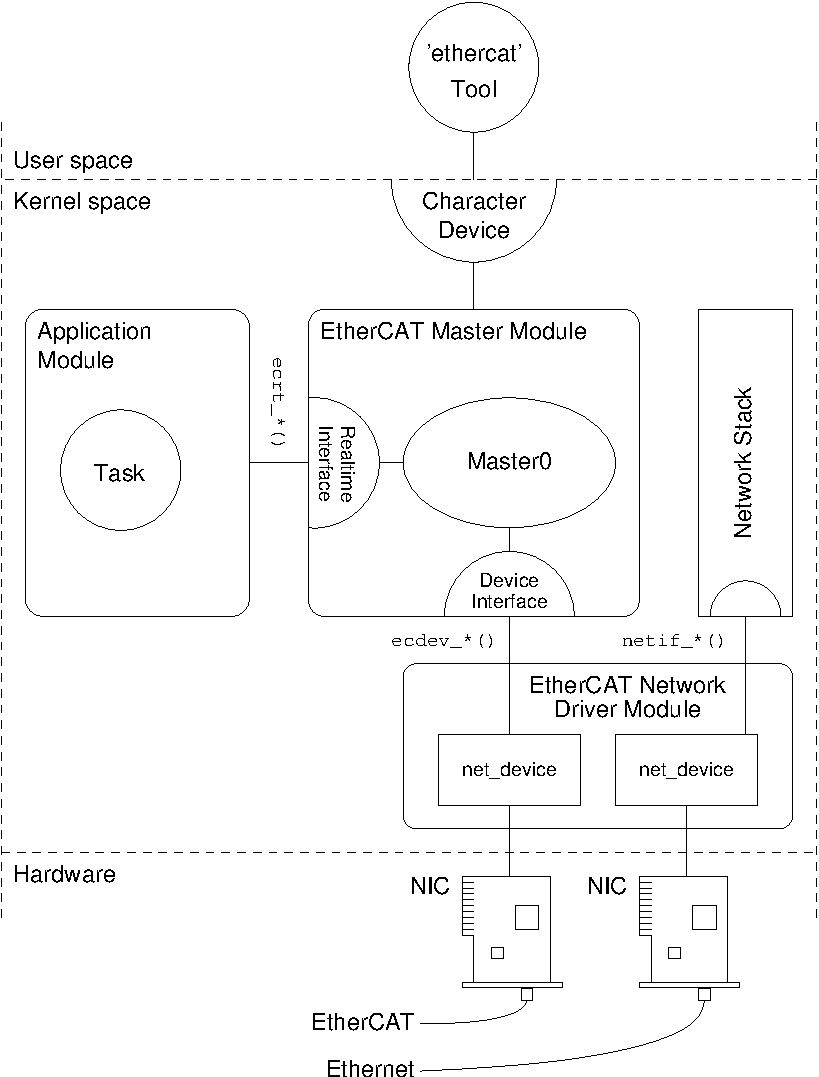
\includegraphics[width=\textwidth]{images/architecture}
  \caption{Master Architecture}
  \label{fig:arch}
\end{figure}

The components of the master environment are described below:

\begin{description}

\item[Master Module]\index{Master Module} Kernel module containing one or more
EtherCAT master instances (see sec.~\ref{sec:mastermod}), the ``Device
Interface'' (see sec.~\ref{sec:ecdev}) and the ``Application Interface'' (see
chap.~\ref{chap:api}).

\item[Device Modules]\index{Device modules} EtherCAT-capable Ethernet device
driver modules\index{Device modules}, that offer their devices to the EtherCAT
master via the device interface (see sec.~\ref{sec:ecdev}). These modified
network drivers can handle network devices used for EtherCAT operation and
``normal'' Ethernet devices in parallel. A master can accept a certain device
and then is able to send and receive EtherCAT frames. Ethernet devices
declined by the master module are connected to the kernel's network stack as
usual.

\item[Application]\index{Application} A program that uses the EtherCAT master
(usually for cyclic exchange of process data with EtherCAT slaves). These
programs are not part of the EtherCAT master code\footnote{Although there are
some examples provided in the \textit{examples/} directory.}, but have to be
generated or written by the user. An application can ``request'' a master
through the application interface (see chap.~\ref{chap:api}). If this
succeeds, it has the control over the master: It can provide a bus
configuration and exchange process data.  Applications can be kernel modules
(that use the kernel application interface directly) or userspace programs,
that use the application interface via the EtherCAT library (see
sec.~\ref{sec:userlib}).

\end{description}

%------------------------------------------------------------------------------

\section{Master Module}
\label{sec:mastermod}
\index{Master module}

The EtherCAT master kernel module \textit{ec\_master} can contain multiple
master instances. Each master waits for a certain Ethernet device identified
by its MAC address\index{MAC address}. These addresses have to be specified on
module loading via the \textit{main\_devices} module parameter. The number of
master instances to initialize is taken from the number of MAC addresses
given.

The below command loads the master module with a single master instance that
waits for the Ethernet device with the MAC address
\lstinline+00:0E:0C:DA:A2:20+. The master will be accessible via index $0$.

\begin{lstlisting}
# `\textbf{modprobe ec\_master main\_devices=00:0E:0C:DA:A2:20}`
\end{lstlisting}

MAC addresses for multiple masters have to be separated by commas:

\begin{lstlisting}
# `\textbf{modprobe ec\_master main\_devices=00:0E:0C:DA:A2:20,00:e0:81:71:d5:1c}`
\end{lstlisting}

The two masters can be addressed by their indices 0 and 1 respectively (see
figure~\ref{fig:masters}). The master index is needed for the
\lstinline+ecrt_master_request()+ function of the application interface (see
chap.~\ref{chap:api}) and the \lstinline+--master+ option of the
\textit{ethercat} command-line tool (see sec.~\ref{sec:tool}), which defaults
to $0$.

\begin{figure}[htbp]
  \centering
  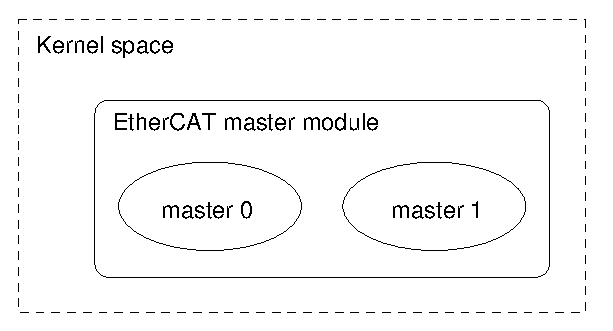
\includegraphics[width=.5\textwidth]{images/masters}
  \caption{Multiple masters in one module}
  \label{fig:masters}
\end{figure}

\paragraph{Debug Level} The master module also has a parameter
\textit{debug\_level} to set the initial debug level for all masters (see
also~\ref{sec:ethercat-debug}).

\paragraph{Init Script}
\index{Init script}

In most cases it is not necessary to load the master module and the Ethernet
driver modules manually. There is an init script available, so the master can
be started as a service (see sec.~\ref{sec:system}).

\paragraph{Syslog}

The master module outputs information about its state and events to the kernel
ring buffer. These also end up in the system logs.  The above module loading
command should result in the messages below:

\begin{lstlisting}
# `\textbf{dmesg | tail -2}`
EtherCAT: Master driver `\masterversion`
EtherCAT: 2 masters waiting for devices.

# `\textbf{tail -2 /var/log/messages}`
Jul  4 10:22:45 ethercat kernel: EtherCAT: Master driver `\masterversion`
Jul  4 10:22:45 ethercat kernel: EtherCAT: 2 masters waiting
                                 for devices.
\end{lstlisting}

All EtherCAT master output is prefixed with \lstinline+EtherCAT+ which makes
searching the logs easier.

%------------------------------------------------------------------------------

\section{Master Phases}
\index{Master phases}

Every EtherCAT master provided by the master module (see
sec.~\ref{sec:mastermod}) runs through several phases (see
fig.~\ref{fig:phases}):

\begin{figure}[htbp]
  \centering
  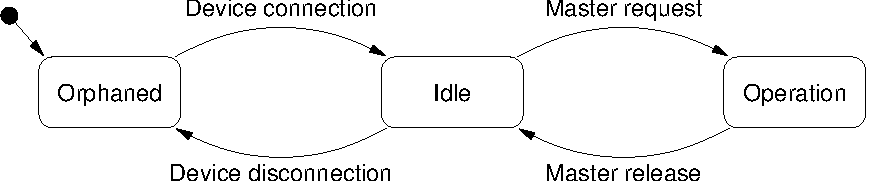
\includegraphics[width=.9\textwidth]{images/phases}
  \caption{Master phases and transitions}
  \label{fig:phases}
\end{figure}

\begin{description}

\item[Orphaned phase]\index{Orphaned phase} This mode takes effect, when the
master still waits for its Ethernet device to connect. No bus communication is
possible until then.

\item[Idle phase]\index{Idle phase} takes effect when the master has accepted
an Ethernet device, but is not requested by any application yet. The master
runs its state machine (see sec.~\ref{sec:fsm-master}), that automatically
scans the bus for slaves and executes pending operations from the userspace
interface (for example SDO access). The command-line tool can be used to
access the bus, but there is no process data exchange because of the missing
bus configuration.

\item[Operation phase]\index{Operation phase} The master is requested by an
application that can provide a bus configuration and exchange process data.

\end{description}

%------------------------------------------------------------------------------

\section{Process Data}
\label{sec:processdata}

This section shall introduce a few terms and ideas how the master handles
process data.

\paragraph{Process Data Image}
\index{Process data}

Slaves offer their inputs and outputs by presenting the master so-called
``Process Data Objects'' (PDOs\index{PDO}). The available PDOs can be either
determined by reading out the slave's TXPDO and RXPDO SII categories from the
E$^2$PROM (in case of fixed PDOs) or by reading out the appropriate CoE
objects (see sec.~\ref{sec:coe}), if available.  The application can register
the PDOs' entries for exchange during cyclic operation. The sum of all
registered PDO entries defines the ``process data image'', which is exchanged
via datagrams with ``logical'' memory access (like LWR, LRD or LRW) introduced
in~\cite[sec.~5.4]{dlspec}.

\paragraph{Process Data Domains}
\index{Domain}

The process data image can be easily managed by creating so-called
``domains'', which allow grouped PDO exchange. They also take care of managing
the datagram structures needed to exchange the PDOs. Domains are mandatory for
process data exchange, so there has to be at least one. They were introduced
for the following reasons:

\begin{itemize}

\item The maximum size of a datagram is limited due to the limited size of an
Ethernet frame: The maximum data size is the Ethernet data field size minus
the EtherCAT frame header, EtherCAT datagram header and EtherCAT datagram
footer: $1500 - 2 - 12 - 2 = 1484$ octets. If the size of the process data
image exceeds this limit, multiple frames have to be sent, and the image has
to be partitioned for the use of multiple datagrams. A domain manages this
automatically.

\item Not every PDO has to be exchanged with the same frequency: The values of
PDOs can vary slowly over time (for example temperature values), so exchanging
them with a high frequency would just waste bus bandwidth. For this reason,
multiple domains can be created, to group different PDOs and so allow separate
exchange.

\end{itemize}

There is no upper limit for the number of domains, but each domain occupies
one FMMU in each slave involved, so the maximum number of domains is de facto
limited by the slaves.

\paragraph{FMMU Configuration}
\index{FMMU!Configuration}

An application can register PDO entries for exchange. Every PDO entry and its
parent PDO is part of a memory area in the slave's physical memory, that is
protected by a sync manager \cite[sec.~6.7]{dlspec} for synchronized access.
In order to make a sync manager react on a datagram accessing its memory, it
is necessary to access the last byte covered by the sync manager. Otherwise
the sync manager will not react on the datagram and no data will be exchanged.
That is why the whole synchronized memory area has to be included into the
process data image: For example, if a certain PDO entry of a slave is
registered for exchange with a certain domain, one FMMU will be configured to
map the complete sync-manager-protected memory, the PDO entry resides in. If a
second PDO entry of the same slave is registered for process data exchange
within the same domain, and it resides in the same sync-manager-protected
memory as the first one, the FMMU configuration is not altered, because the
desired memory is already part of the domain's process data image. If the
second PDO entry would belong to another sync-manager-protected area, this
complete area would also be included into the domains process data image.

Figure~\ref{fig:fmmus} gives an overview, how FMMUs are configured to map
physical memory to logical process data images.

\begin{figure}[htbp]
  \centering
  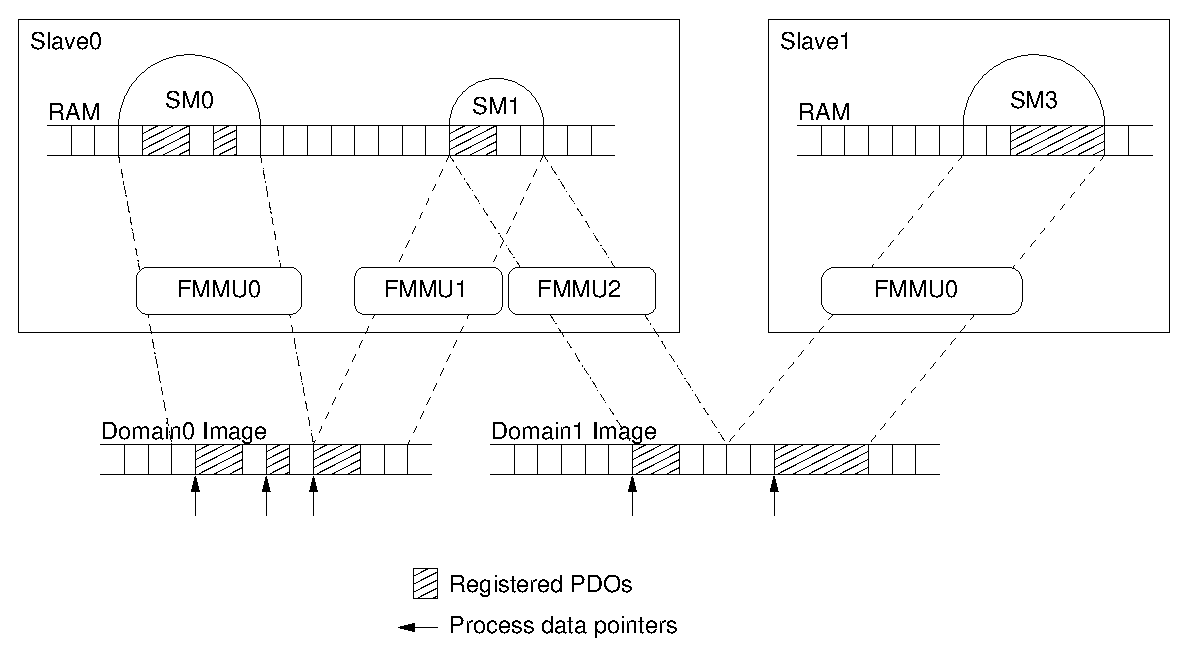
\includegraphics[width=\textwidth]{images/fmmus}
  \caption{FMMU Configuration}
  \label{fig:fmmus}
\end{figure}

%------------------------------------------------------------------------------

\chapter{Application Interface}
\label{chap:api}
\index{Application interface}

% TODO
%
% Interface version
% Master Requesting and Releasing
% Master Locking
% Configuring PDO assignment and mapping
% Domains (memory)
% PDO entry registration
% SDO configuration
% SDO access
% IDN configurations
% IDN access

The application interface provides functions and data structures for
applications to access an EtherCAT master. The complete documentation of the
interface is included as Doxygen~\cite{doxygen} comments in the header file
\textit{include/ecrt.h}. It can either be read directly from the file
comments, or as a more comfortable HTML documentation. The HTML generation is
described in sec.~\ref{sec:gendoc}.

The following sections cover a general description of the application
interface.

Every application should use the master in two steps:

\begin{description}

\item[Configuration] The master is requested and the configuration is applied.
For example, domains are created, slaves are configured and PDO entries are
registered (see sec.~\ref{sec:masterconfig}).

\item[Operation] Cyclic code is run and process data are exchanged (see
sec.~\ref{sec:cyclic}).

\end{description}

\paragraph{Example Applications}\index{Example Applications} There are a few
example applications in the \textit{examples/} subdirectory of the master
code. They are documented in the source code.

%------------------------------------------------------------------------------

\section{Master Configuration}
\label{sec:masterconfig}

The bus configuration is supplied via the application interface.
Figure~\ref{fig:app-config} gives an overview of the objects, that can be
configured by the application.

\begin{figure}[htbp]
  \centering
  \includegraphics[width=.8\textwidth]{images/app-config}
  \caption{Master Configuration}
  \label{fig:app-config}
\end{figure}

\subsection{Slave Configuration}

The application has to tell the master about the expected bus topology. This
can be done by creating ``slave configurations''. A slave configuration can be
seen as an expected slave. When a slave configuration is created, the
application provides the bus position (see below), vendor id and product code.

When the bus configuration is applied, the master checks, if there is a slave
with the given vendor id and product code at the given position. If this is
the case, the slave configuration is ``attached'' to the real slave on the bus
and the slave is configured according to the settings provided by the
application. The state of a slave configuration can either be queried via the
application interface or via the command-line tool (see
sec.~\ref{sec:ethercat-config}).

\paragraph{Slave Position} The slave position has to be specified as a tuple
of ``alias'' and ``position''. This allows addressing slaves either via an
absolute bus position, or a stored identifier called ``alias'', or a mixture
of both. The alias is a 16-bit value stored in the slave's E$^2$PROM. It can
be modified via the command-line tool (see sec.~\ref{sec:ethercat-alias}).
Table~\ref{tab:slaveposition} shows, how the values are interpreted.

\begin{table}[htbp]
  \centering
  \caption{Specifying a Slave Position}
  \label{tab:slaveposition}
  \vspace{2mm}
  \begin{tabular}{c|c|p{70mm}}
    Alias & Position & Interpretation\\
    \hline

    \lstinline+0+ & \lstinline+0+ -- \lstinline+65535+ &

    Position addressing. The position parameter is interpreted as the absolute
    ring position in the bus.\\ \hline

    \lstinline+1+ -- \lstinline+65535+ & \lstinline+0+ -- \lstinline+65535+ &

    Alias addressing. The position parameter is interpreted as relative
    position after the first slave with the given alias address. \\ \hline

  \end{tabular}
\end{table}

Figure~\ref{fig:attach} shows an example of how slave configurations are
attached. Some of the configurations were attached, while others remain
detached. The below lists gives the reasons beginning with the top slave
configuration.

\begin{figure}[htbp]
  \centering
  \includegraphics[width=.7\textwidth]{images/attach}
  \caption{Slave Configuration Attachment}
  \label{fig:attach}
\end{figure}

\begin{enumerate}

\item A zero alias means to use simple position addressing. Slave 1 exists and
vendor id and product code match the expected values.

\item Although the slave with position 0 is found, the product code does not
match, so the configuration is not attached.

\item The alias is non-zero, so alias addressing is used. Slave 2 is the first
slave with alias \lstinline+0x2000+. Because the position value is zero, the
same slave is used.

\item There is no slave with the given alias, so the configuration can not be
attached.

\item Slave 2 is again the first slave with the alias \lstinline+0x2000+, but
position is now 1, so slave 3 is attached.

\end{enumerate}

%------------------------------------------------------------------------------

\section{Cyclic Operation}
\label{sec:cyclic}


To enter cyclic operation mode, the master has to be ``activated'' to
calculate the process data image and apply the bus configuration for the first
time. After activation, the application is in charge to send and receive
frames.

% TODO
%
% PDO endianess
% Datagram injection

%------------------------------------------------------------------------------

\section{VoE Handlers}
\label{sec:api-voe}

During the configuration phase, the application can create handlers for the
VoE mailbox protocol described in sec.~\ref{sec:voe}. One VoE handler always
belongs to a certain slave configuration, so the creation function is a method
of the slave configuration.

A VoE handler manages the VoE data and the datagram used to transmit and
receive VoE messages. Is contains the state machine necessary to transfer VoE
messages.

The VoE state machine can only process one operation at a time. As a result,
either a read or write operation may be issued at a time\footnote{If
simultaneous sending and receiving is desired, two VoE handlers can be created
for the slave configuration.}. After the operation is initiated, the handler
must be executed cyclically until it is finished. After that, the results of
the operation can be retrieved.

A VoE handler has an own datagram structure, that is marked for exchange after
each execution step. So the application can decide, how many handlers to
execute before sending the corresponding EtherCAT frame(s).

For more information about the use of VoE handlers see the documentation of
the application interface functions and the example applications provided in
the \textit{examples/} directory.

%------------------------------------------------------------------------------

\section{Concurrent Master Access}
\label{sec:concurr}
\index{Concurrency}

In some cases, one master is used by several instances, for example when an
application does cyclic process data exchange, and there are EoE-capable
slaves that require to exchange Ethernet data with the kernel (see
sec.~\ref{sec:eoe}). For this reason, the master is a shared resource, and
access to it has to be sequentialized. This is usually done by locking with
semaphores, or other methods to protect critical sections.

The master itself can not provide locking mechanisms, because it has no chance
to know the appropriate kind of lock. For example if the application is in
kernelspace and uses RTAI functionality, ordinary kernel semaphores would not
be sufficient. For that, an important design decision was made: The
application that reserved a master must have the total control, therefore it
has to take responsibility for providing the appropriate locking mechanisms.
If another instance wants to access the master, it has to request the bus
access via callbacks, that have to be provided by the application. Moreover
the application can deny access to the master if it considers it to be awkward
at the moment.

\begin{figure}[htbp]
  \centering
  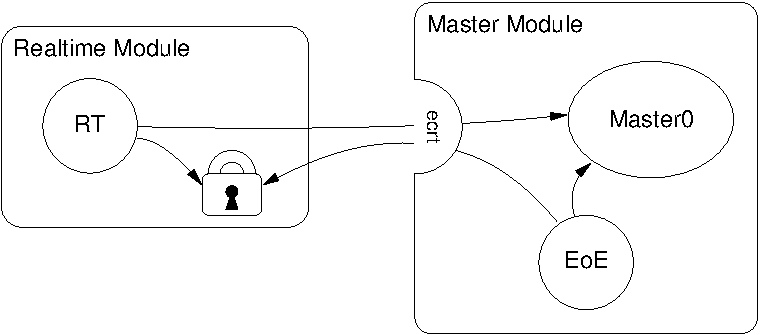
\includegraphics[width=.6\textwidth]{images/master-locks}
  \caption{Concurrent Master Access}
  \label{fig:locks}
\end{figure}

Figure~\ref{fig:locks} exemplary shows, how two processes share one master:
The application's cyclic task uses the master for process data exchange, while
the master-internal EoE process uses it to communicate with EoE-capable
slaves. Both have to access the bus from time to time, but the EoE process
does this by ``asking'' the application to do the bus access for it. In this
way, the application can use the appropriate locking mechanism to avoid
accessing the bus at the same time. See the application interface
documentation (chap.~\ref{chap:api}) for how to use these callbacks.

%------------------------------------------------------------------------------

\section{Distributed Clocks}
\label{sec:dc}
\index{Distributed Clocks}

From version 1.5, the master supports EtherCAT's ``Distributed Clocks''
feature. It is possible to synchronize the slave clocks on the bus to the
``reference clock'' (which is the local clock of the first slave with DC
support) and to synchronize the reference clock to the ``master clock'' (which
is the local clock of the master). All other clocks on the bus (after the
reference clock) are considered as ``slave clocks'' (see fig.~\ref{fig:dc}).

\begin{figure}[htbp]
  \centering
  \includegraphics[width=.8\textwidth]{images/dc}
  \caption{Distributed Clocks}
  \label{fig:dc}
\end{figure}

\paragraph{Local Clocks} Any EtherCAT slave that supports DC has a local clock
register with nanosecond resolution. If the slave is powered, the clock starts
from zero, meaning that when slaves are powered on at different times, their
clocks will have different values. These ``offsets'' have to be compensated by
the distributed clocks mechanism. On the other hand, the clocks do not run
exactly with the same speed, since the used quarts units have a natural
frequency deviation. This deviation is usually very small, but over longer
periods, the error would accumulate and the difference between local clocks
would grow. This clock ``drift'' has also to be compensated by the DC
mechanism.

\paragraph{Application Time} The common time base for the bus has to be
provided by the application. This application time $t_\text{app}$ is used

\begin{enumerate}
\item to configure the slaves' clock offsets (see below),
\item to program the slave's start times for sync pulse generation (see
below).
\item to synchronize the reference clock to the master clock (optional).
\end{enumerate}

\paragraph{Offset Compensation} For the offset compensation, each slave
provides a ``System Time Offset'' register $t_\text{off}$, that is added to
the internal clock value $t_\text{int}$ to get the ``System Time''
$t_\text{sys}$:

\begin{eqnarray}
t_\text{sys} & = & t_\text{int} + t_\text{off} \\
\Rightarrow t_\text{int} & = & t_\text{sys} - t_\text{off} \nonumber
\end{eqnarray}

The master reads the values of both registers to calculate a new system time
offset in a way, that the resulting system time shall match the master's
application time $t_\text{app}$:

\begin{eqnarray}
t_\text{sys} & \stackrel{!}{=} & t_\text{app} \\
\Rightarrow t_\text{int} + t_\text{off} & \stackrel{!}{=} & t_\text{app} \nonumber \\
\Rightarrow t_\text{off} & = & t_\text{app} - t_\text{int} \nonumber \\
\Rightarrow t_\text{off} & = & t_\text{app} - (t_\text{sys} - t_\text{off}) \nonumber \\
\Rightarrow t_\text{off} & = & t_\text{app} - t_\text{sys} + t_\text{off}
\end{eqnarray}

The small time offset error resulting from the different times of reading and
writing the registers will be compensated by the drift compensation.

\paragraph{Drift Compensation} The drift compensation is possible due to a
special mechanism in each DC-capable slave: A write operation to the ``System
time'' register will cause the internal time control loop to compare the
written time (minus the programmed transmission delay, see below) to the
current system time. The calculated time error will be used as an input to the
time controller, that will tune the local clock speed to be a little faster or
slower\footnote{The local slave clock will be incremented either with
\unit{9}{\nano\second}, \unit{10}{\nano\second} or \unit{11}{\nano\second}
every \unit{10}{\nano\second}.}, according to the sign of the error.

\paragraph{Transmission Delays} The Ethernet frame needs a small amount of
time to get from slave to slave. The resulting transmission delay times
accumulate on the bus and can reach microsecond magnitude and thus have to be
considered during the drift compensation. EtherCAT slaves supporting DC
provide a mechanism to measure the transmission delays: For each of the four
slave ports there is a receive time register. A write operation to the receive
time register of port 0 starts the measuring and the current system time is
latched and stored in a receive time register once the frame is received on
the corresponding port. The master can read out the relative receive times,
then calculate time delays between the slaves (using its knowledge of the bus
topology), and finally calculate the time delays from the reference clock to
each slave. These values are programmed into the slaves' transmission delay
registers. In this way, the drift compensation can reach nanosecond synchrony. 

\paragraph{Checking Synchrony} DC-capable slaves provide the 32-bit ``System
time difference'' register at address \lstinline+0x092c+, where the system
time difference of the last drift compensation is stored in nanosecond
resolution and in sign-and-magnitude coding\footnote{This allows
broadcast-reading all system time difference registers on the bus to get an
upper approximation}. To check for bus synchrony, the system time difference
registers can also be cyclically read via the command-line-tool (see
sec.~\ref{sec:regaccess}):

\begin{lstlisting}
$ `\textbf{watch -n0 "ethercat reg\_read -p4 -tsm32 0x92c"}`
\end{lstlisting}

\paragraph{Sync Signals} Synchronous clocks are only the prerequisite for
synchronous events on the bus. Each slave with DC support provides two ``sync
signals'', that can be programmed to create events, that will for example
cause the slave application to latch its inputs on a certain time. A sync
event can either be generated once or cyclically, depending on what makes
sense for the slave application. Programming the sync signals is a matter of
setting the so-called ``AssignActivate'' word and the sync signals' cycle- and
shift times. The AssignActivate word is slave-specific and has to be taken
from the XML slave description (\lstinline+Device+ $\rightarrow$
\lstinline+Dc+), where also typical sync signal configurations ``OpModes'' can
be found.

%------------------------------------------------------------------------------

\chapter{Ethernet Devices}
\label{sec:devices}

The EtherCAT protocol is based on the Ethernet standard, so a master relies on
standard Ethernet hardware to communicate with the bus.

The term \textit{device} is used as a synonym for Ethernet network interface
hardware.

\paragraph{Native Ethernet Device Drivers} There are native device driver
modules (see sec.~\ref{sec:native-drivers}) that handle Ethernet hardware,
which a master can use to connect to an EtherCAT bus. They offer their
Ethernet hardware to the master module via the device interface (see
sec.~\ref{sec:ecdev}) and must be capable to prepare Ethernet devices either
for EtherCAT (realtime) operation or for ``normal'' operation using the
kernel's network stack. The advantage of this approach is that the master can
operate nearly directly on the hardware, which allows a high performance. The
disadvantage is, that there has to be an EtherCAT-capable version of the
original Ethernet driver.

\paragraph{Generic Ethernet Device Driver} From master version 1.5, there is a
generic Ethernet device driver module (see sec.~\ref{sec:generic-driver}),
that uses the lower layers of the network stack to connect to the hardware.
The advantage is, that arbitrary Ethernet hardware can be used for EtherCAT
operation, independently of the actual hardware driver (so all Linux Ethernet
drivers are supported without modifications). The disadvantage is, that this
approach does not support realtime extensions like RTAI, because the Linux
network stack is addressed. Moreover the performance is a little worse than
the native approach, because the Ethernet frame data have to traverse the
network stack.

%------------------------------------------------------------------------------

\section{Network Driver Basics}
\label{sec:networkdrivers}
\index{Network drivers}

EtherCAT relies on Ethernet hardware and the master needs a physical
Ethernet device to communicate with the bus. Therefore it is necessary
to understand how Linux handles network devices and their drivers,
respectively.

\paragraph{Tasks of a Network Driver} Network device drivers usually handle
the lower two layers of the OSI model, that is the physical layer and the
data-link layer. A network device itself natively handles the physical layer
issues: It represents the hardware to connect to the medium and to send and
receive data in the way, the physical layer protocol describes. The network
device driver is responsible for getting data from the kernel's networking
stack and forwarding it to the hardware, that does the physical transmission.
If data is received by the hardware respectively, the driver is notified
(usually by means of an interrupt) and has to read the data from the hardware
memory and forward it to the network stack. There are a few more tasks, a
network device driver has to handle, including queue control, statistics and
device dependent features.

\paragraph{Driver Startup} Usually, a driver searches for compatible devices
on module loading.  For PCI drivers, this is done by scanning the PCI bus and
checking for known device IDs. If a device is found, data structures are
allocated and the device is taken into operation.

\paragraph{Interrupt Operation}\index{Interrupt} A network device usually
provides a hardware interrupt that is used to notify the driver of received
frames and success of transmission, or errors, respectively. The driver has to
register an interrupt service routine
(ISR\index{ISR}\nomenclature{ISR}{Interrupt Service Routine}), that is
executed each time, the hardware signals such an event. If the interrupt was
thrown by the own device (multiple devices can share one hardware interrupt),
the reason for the interrupt has to be determined by reading the device's
interrupt register. For example, if the flag for received frames is set, frame
data has to be copied from hardware to kernel memory and passed to the network
stack.

\paragraph{The \lstinline+net_device+ Structure}\index{net\_device} The driver
registers a \lstinline+net_device+ structure for each device to communicate
with the network stack and to create a ``network interface''. In case of an
Ethernet driver, this interface appears as \textit{ethX}, where X is a number
assigned by the kernel on registration. The \lstinline+net_device+ structure
receives events (either from userspace or from the network stack) via several
callbacks, which have to be set before registration. Not every callback is
mandatory, but for reasonable operation the ones below are needed in any case:

\newsavebox\boxopen
\sbox\boxopen{\lstinline+open()+}
\newsavebox\boxstop
\sbox\boxstop{\lstinline+stop()+}
\newsavebox\boxxmit
\sbox\boxxmit{\lstinline+hard_start_xmit()+}
\newsavebox\boxstats
\sbox\boxstats{\lstinline+get_stats()+}

\begin{description}

\item[\usebox\boxopen] This function is called when network communication has
to be started, for example after a command \lstinline+ip link set ethX up+
from userspace. Frame reception has to be enabled by the driver.

\item[\usebox\boxstop] The purpose of this callback is to ``close'' the
device, i.\,e.\ make the hardware stop receiving frames.

\item[\usebox\boxxmit] This function is called for each frame that has to be
transmitted. The network stack passes the frame as a pointer to an
\lstinline+sk_buff+ structure (``socket buffer''\index{Socket buffer}, see
below), which has to be freed after sending.

\item[\usebox\boxstats] This call has to return a pointer to the device's
\lstinline+net_device_stats+ structure, which permanently has to be filled with
frame statistics. This means, that every time a frame is received, sent, or an
error happened, the appropriate counter in this structure has to be increased.

\end{description}

The actual registration is done with the \lstinline+register_netdev()+ call,
unregistering is done with \lstinline+unregister_netdev()+.

\paragraph{The \lstinline+netif+ Interface}\index{netif} All other
communication in the direction interface $\to$ network stack is done via the
\lstinline+netif_*()+ calls. For example, on successful device opening, the
network stack has to be notified, that it can now pass frames to the
interface. This is done by calling \lstinline+netif_start_queue()+. After this
call, the \lstinline+hard_start_xmit()+ callback can be called by the network
stack. Furthermore a network driver usually manages a frame transmission
queue.  If this gets filled up, the network stack has to be told to stop
passing further frames for a while. This happens with a call to
\lstinline+netif_stop_queue()+. If some frames have been sent, and there is
enough space again to queue new frames, this can be notified with
\lstinline+netif_wake_queue()+. Another important call is
\lstinline+netif_receive_skb()+\footnote{This function is part of the NAPI
(``New API''), that replaces the kernel 2.4 technique for interfacing to the
network stack (with \lstinline+netif_rx()+). NAPI is a technique to improve
network performance on Linux. Read more in
\url{http://www.cyberus.ca/~hadi/usenix-paper.tgz}.}: It passes a frame to the
network stack, that was just received by the device. Frame data has to be
included in a so-called ``socket buffer'' for that (see below).

\paragraph{Socket Buffers}\index{Socket buffer} Socket buffers are the basic
data type for the whole network stack. They serve as containers for network
data and are able to quickly add data headers and footers, or strip them off
again. Therefore a socket buffer consists of an allocated buffer and several
pointers that mark beginning of the buffer (\lstinline+head+), beginning of
data (\lstinline+data+), end of data (\lstinline+tail+) and end of buffer
(\lstinline+end+). In addition, a socket buffer holds network header
information and (in case of received data) a pointer to the
\lstinline+net_device+, it was received on. There exist functions that create
a socket buffer (\lstinline+dev_alloc_skb()+), add data either from front
(\lstinline+skb_push()+) or back (\lstinline+skb_put()+), remove data from
front (\lstinline+skb_pull()+) or back (\lstinline+skb_trim()+), or delete the
buffer (\lstinline+kfree_skb()+).  A socket buffer is passed from layer to
layer, and is freed by the layer that uses it the last time. In case of
sending, freeing has to be done by the network driver.

%------------------------------------------------------------------------------

\section{Native EtherCAT Device Drivers}
\label{sec:native-drivers}

There are a few requirements, that applies to Ethernet hardware when used with
a native Ethernet driver with EtherCAT functionality.

\paragraph{Dedicated Hardware} For performance and realtime purposes, the
EtherCAT master needs direct and exclusive access to the Ethernet hardware.
This implies that the network device must not be connected to the kernel's
network stack as usual, because the kernel would try to use it as an ordinary
Ethernet device.

\paragraph{Interrupt-less Operation}\index{Interrupt} EtherCAT frames travel
through the logical EtherCAT ring and are then sent back to the master.
Communication is highly deterministic: A frame is sent and will be received
again after a constant time, so there is no need to notify the driver about
frame reception: The master can instead query the hardware for received
frames, if it expects them to be already received.

Figure~\ref{fig:interrupt} shows two workflows for cyclic frame transmission
and reception with and without interrupts.

\begin{figure}[htbp]
  \centering
  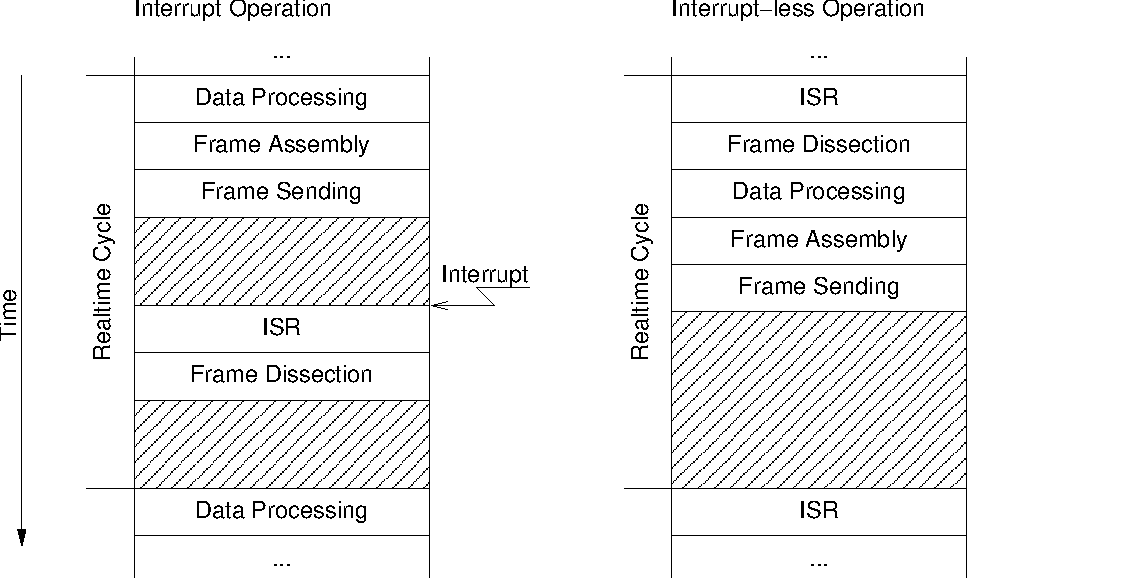
\includegraphics[width=.9\textwidth]{images/interrupt}
  \caption{Interrupt Operation versus Interrupt-less Operation}
  \label{fig:interrupt}
\end{figure}

In the left workflow ``Interrupt Operation'', the data from the last cycle is
first processed and a new frame is assembled with new datagrams, which is then
sent.  The cyclic work is done for now.  Later, when the frame is received
again by the hardware, an interrupt is triggered and the ISR is executed. The
ISR will fetch the frame data from the hardware and initiate the frame
dissection: The datagrams will be processed, so that the data is ready for
processing in the next cycle.

In the right workflow ``Interrupt-less Operation'', there is no hardware
interrupt enabled.  Instead, the hardware will be polled by the master by
executing the ISR. If the frame has been received in the meantime, it will be
dissected. The situation is now the same as at the beginning of the left
workflow: The received data is processed and a new frame is assembled and
sent. There is nothing to do for the rest of the cycle.

The interrupt-less operation is desirable, because hardware interrupts are not
conducive in improving the driver's realtime behaviour: Their indeterministic
incidences contribute to increasing the jitter. Besides, if a realtime
extension (like RTAI) is used, some additional effort would have to be made to
prioritize interrupts.

\paragraph{Ethernet and EtherCAT Devices} Another issue lies in the way Linux
handles devices of the same type.  For example, a
PCI\nomenclature{PCI}{Peripheral Component Interconnect, Computer Bus} driver
scans the PCI bus for devices it can handle. Then it registers itself as the
responsible driver for all of the devices found. The problem is, that an
unmodified driver can not be told to ignore a device because it will be used
for EtherCAT later. There must be a way to handle multiple devices of the same
type, where one is reserved for EtherCAT, while the other is treated as an
ordinary Ethernet device.

For all this reasons, the author decided that the only acceptable solution is
to modify standard Ethernet drivers in a way that they keep their normal
functionality, but gain the ability to treat one or more of the devices as
EtherCAT-capable.

Below are the advantages of this solution:

\begin{itemize}
\item No need to tell the standard drivers to ignore certain devices.
\item One networking driver for EtherCAT and non-EtherCAT devices.
\item No need to implement a network driver from scratch and running
  into issues, the former developers already solved.
\end{itemize}

The chosen approach has the following disadvantages:

\begin{itemize}
\item The modified driver gets more complicated, as it must handle
  EtherCAT and non-EtherCAT devices.
\item Many additional case differentiations in the driver code.
\item Changes and bug fixes on the standard drivers have to be ported
  to the Ether\-CAT-capable versions from time to time.
\end{itemize}

%------------------------------------------------------------------------------

\section{Generic EtherCAT Device Driver}
\label{sec:generic-driver}

Since there are approaches to enable the complete Linux kernel for realtime
operation \cite{rt-preempt}, it is possible to operate without native
implementations of EtherCAT-capable Ethernet device drivers and use the Linux
network stack instead. Fig.~\ref{fig:arch} shows the ``Generic Ethernet Driver
Module'', that connects to local Ethernet devices via the network stack. The
kernel module is named \lstinline+ec_generic+ and can be loaded after the
master module like a native EtherCAT-capable Ethernet driver.

The generic device driver scans the network stack for interfaces, that have
been registered by Ethernet device drivers. It offers all possible devices to
the EtherCAT master. If the master accepts a device, the generic driver
creates a packet socket (see \lstinline+man 7 packet+) with
\lstinline+socket_type+ set to \lstinline+SOCK_RAW+, bound to that device. All
functions of the device interface (see sec.~\ref{sec:ecdev}) will then operate
on that socket.

Below are the advantages of this solution:

\begin{itemize}
\item Any Ethernet hardware, that is covered by a Linux Ethernet driver can be
used for EtherCAT.
\item No modifications have to be made to the actual Ethernet drivers.
\end{itemize}

The generic approach has the following disadvantages:

\begin{itemize}
\item The performance is a little worse than the native approach, because the
frame data have to traverse the lower layers of the network stack.
\item It is not possible to use in-kernel realtime extensions like RTAI with
the generic driver, because the network stack code uses dynamic memory
allocations and other things, that could cause the system to freeze in
realtime context.
\end{itemize}

%------------------------------------------------------------------------------

\section{Providing Ethernet Devices}
\label{sec:providing-devices}

After loading the master module, additional module(s) have to be loaded to
offer devices to the master(s) (see sec.~\ref{sec:ecdev}). The master module
knows the devices to choose from the module parameters (see
sec.~\ref{sec:mastermod}). If the init script is used to start the master, the
drivers and devices to use can be specified in the sysconfig file (see
sec.~\ref{sec:sysconfig}).

Modules offering Ethernet devices can be

\begin{itemize}
\item native EtherCAT-capable network driver modules (see
sec.~\ref{sec:native-drivers}) or
\item the generic EtherCAT device driver module (see
sec.~\ref{sec:generic-driver}).
\end{itemize}

%------------------------------------------------------------------------------

\section{EtherCAT Device Interface}
\label{sec:ecdev}
\index{Device interface}

An anticipation to the section about the master module
(sec.~\ref{sec:mastermod}) has to be made in order to understand the way, a
network device driver module can connect a device to a specific EtherCAT
master.

The master module provides a ``device interface'' for network device drivers.
To use this interface, a network device driver module must include the header
\textit{devices/ecdev.h}\nomenclature{ecdev}{EtherCAT Device}, coming with the
EtherCAT master code. This header offers a function interface for EtherCAT
devices. All functions of the device interface are named with the prefix
\lstinline+ecdev+.

The documentation of the device interface can be found in the header file or
in the appropriate module of the interface documentation (see
sec.~\ref{sec:gendoc} for generation instructions).

% TODO general description of the device interface

%------------------------------------------------------------------------------

\section{Patching Native Network Drivers}
\label{sec:patching}
\index{Network drivers}

This section will describe, how to make a standard Ethernet driver
EtherCAT-capable, using the native approach (see
sec.~\ref{sec:native-drivers}). Unfortunately, there is no standard procedure
to enable an Ethernet driver for use with the EtherCAT master, but there are a
few common techniques.

\begin{enumerate}

\item A first simple rule is, that \lstinline+netif_*()+ calls must be avoided
for all EtherCAT devices. As mentioned before, EtherCAT devices have no
connection to the network stack, and therefore must not call its interface
functions.

\item Another important thing is, that EtherCAT devices should be operated
without interrupts. So any calls of registering interrupt handlers and enabling
interrupts at hardware level must be avoided, too.

\item The master does not use a new socket buffer for each send operation:
Instead there is a fix one allocated on master initialization. This socket
buffer is filled with an EtherCAT frame with every send operation and passed to
the \lstinline+hard_start_xmit()+ callback. For that it is necessary, that the
socket buffer is not be freed by the network driver as usual.

\end{enumerate}

An Ethernet driver usually handles several Ethernet devices, each described by
a \lstinline+net_device+ structure with a \lstinline+priv_data+ field to
attach driver-dependent data to the structure. To distinguish between normal
Ethernet devices and the ones used by EtherCAT masters, the private data
structure used by the driver could be extended by a pointer, that points to an
\lstinline+ec_device_t+ object returned by \lstinline+ecdev_offer()+ (see
sec.~\ref{sec:ecdev}) if the device is used by a master and otherwise is zero.

The RealTek RTL-8139 Fast Ethernet driver is a ``simple'' Ethernet driver and
can be taken as an example to patch new drivers. The interesting sections can
be found by searching the string ``ecdev" in the file
\textit{devices/8139too-2.6.24-ethercat.c}.

%------------------------------------------------------------------------------

\chapter{State Machines}
\label{sec:fsm}
\index{FSM}

Many parts of the EtherCAT master are implemented as \textit{finite state
machines} (FSMs\nomenclature{FSM}{Finite State Machine}). Though this leads
to a higher grade of complexity in some aspects, is opens many new
possibilities.

The below short code example exemplary shows how to read all slave
states and moreover illustrates the restrictions of ``sequential''
coding:

\begin{lstlisting}[gobble=2,language=C,numbers=left]
  ec_datagram_brd(datagram, 0x0130, 2); // prepare datagram
  if (ec_master_simple_io(master, datagram)) return -1;
  slave_states = EC_READ_U8(datagram->data); // process datagram
\end{lstlisting}

The \textit{ec\_master\_simple\_io()} function provides a simple interface for
synchronously sending a single datagram and receiving the result\footnote{For
all communication issues have been meanwhile sourced out into state machines,
the function is deprecated and stopped existing. Nevertheless it is adequate
for showing it's own restrictions.}. Internally, it queues the specified
datagram, invokes the \textit{ec\_master\_send\_datagrams()} function to send
a frame with the queued datagram and then waits actively for its reception.

This sequential approach is very simple, reflecting in only three lines of
code. The disadvantage is, that the master is blocked for the time it waits
for datagram reception. There is no difficulty when only one instance is using
the master, but if more instances want to (synchronously\footnote{At this
time, synchronous master access will be adequate to show the advantages of an
FSM. The asynchronous approach will be discussed in sec.~\ref{sec:eoe}}) use
the master, it is inevitable to think about an alternative to the sequential
model.

Master access has to be sequentialized for more than one instance
wanting to send and receive datagrams synchronously. With the present
approach, this would result in having one phase of active waiting for
each instance, which would be non-acceptable especially in realtime
circumstances, because of the huge time overhead.

A possible solution is, that all instances would be executed
sequentially to queue their datagrams, then give the control to the
next instance instead of waiting for the datagram reception. Finally,
bus IO is done by a higher instance, which means that all queued
datagrams are sent and received. The next step is to execute all
instances again, which then process their received datagrams and issue
new ones.

This approach results in all instances having to retain their state,
when giving the control back to the higher instance. It is quite
obvious to use a \textit{finite state machine} model in this case.
Section~\ref{sec:fsmtheory} will introduce some of the theory used,
while the listings below show the basic approach by coding the example
from above as a state machine:

\begin{lstlisting}[gobble=2,language=C,numbers=left]
  // state 1
  ec_datagram_brd(datagram, 0x0130, 2); // prepare datagram
  ec_master_queue(master, datagram); // queue datagram
  next_state = state_2;
  // state processing finished
\end{lstlisting}

After all instances executed their current state and queued their
datagrams, these are sent and received. Then the respective next
states are executed:

\begin{lstlisting}[gobble=2,language=C,numbers=left]
  // state 2
  if (datagram->state != EC_DGRAM_STATE_RECEIVED) {
          next_state = state_error;
          return; // state processing finished
  }
  slave_states = EC_READ_U8(datagram->data); // process datagram
  // state processing finished.
\end{lstlisting}

See sec.~\ref{sec:statemodel} for an introduction to the state machine
programming concept used in the master code.

%------------------------------------------------------------------------------

\section{State Machine Theory}
\label{sec:fsmtheory}
\index{FSM!Theory}

A finite state machine \cite{automata} is a model of behavior with
inputs and outputs, where the outputs not only depend on the inputs,
but the history of inputs. The mathematical definition of a finite
state machine (or finite automaton) is a six-tuple $(\Sigma, \Gamma,
S, s_0, \delta, \omega)$, with

\begin{itemize}
\item the input alphabet $\Sigma$, with $\Sigma \neq
  \emptyset$, containing all input symbols,
\item the output alphabet $\Gamma$, with $\Gamma \neq
  \emptyset$, containing all output symbols,
\item the set of states $S$, with $S \neq \emptyset$,
\item the set of initial states $s_0$ with $s_0 \subseteq S, s_0 \neq
  \emptyset$
\item the transition function $\delta: S \times \Sigma \rightarrow S
  \times \Gamma$
\item the output function $\omega$.
\end{itemize}

The state transition function $\delta$ is often specified by a
\textit{state transition table}, or by a \textit{state transition
  diagram}. The transition table offers a matrix view of the state
machine behavior (see table~\ref{tab:statetrans}). The matrix rows
correspond to the states ($S = \{s_0, s_1, s_2\}$) and the columns
correspond to the input symbols ($\Gamma = \{a, b, \varepsilon\}$).
The table contents in a certain row $i$ and column $j$ then represent
the next state (and possibly the output) for the case, that a certain
input symbol $\sigma_j$ is read in the state $s_i$.

\begin{table}[htbp]
  \caption{A typical state transition table}
  \label{tab:statetrans}
  \vspace{2mm}
  \centering
  \begin{tabular}{l|ccc}
    & $a$ & $b$ & $\varepsilon$\\ \hline
    $s_0$ & $s_1$ & $s_1$ & $s_2$\\
    $s_1$ & $s_2$ & $s_1$ & $s_0$\\
    $s_2$ & $s_0$ & $s_0$ & $s_0$\\ \hline
  \end{tabular}
\end{table}

The state diagram for the same example looks like the one in
figure~\ref{fig:statetrans}. The states are represented as circles or
ellipses and the transitions are drawn as arrows between them. Close
to a transition arrow can be the condition that must be fulfilled to
allow the transition. The initial state is marked by a filled black
circle with an arrow pointing to the respective state.

\begin{figure}[htbp]
  \centering
  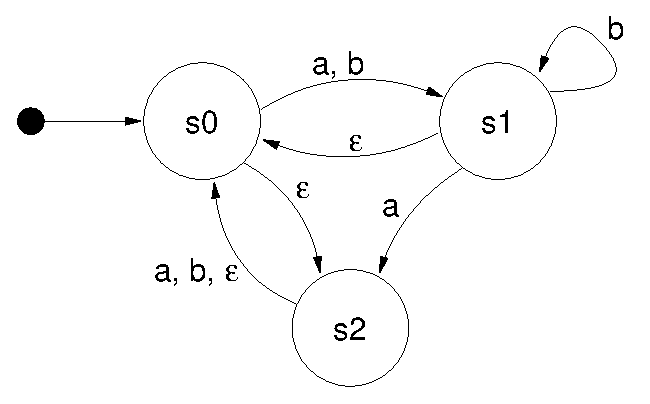
\includegraphics[width=.5\textwidth]{images/statetrans}
  \caption{A typical state transition diagram}
  \label{fig:statetrans}
\end{figure}

\paragraph{Deterministic and non-deterministic state machines}

A state machine can be deterministic, meaning that for one state and
input, there is one (and only one) following state. In this case, the
state machine has exactly one starting state. Non-deterministic state
machines can have more than one transitions for a single state-input
combination. There is a set of starting states in the latter case.

\paragraph{Moore and Mealy machines}

There is a distinction between so-called \textit{Moore machines}, and
\textit{Mealy machines}. Mathematically spoken, the distinction lies
in the output function $\omega$: If it only depends on the current
state ($\omega: S \rightarrow \Gamma$), the machine corresponds to the
``Moore Model''. Otherwise, if $\omega$ is a function of a state and
the input alphabet ($\omega: S \times \Sigma \rightarrow \Gamma$) the
state machine corresponds to the ``Mealy model''. Mealy machines are
the more practical solution in most cases, because their design allows
machines with a minimum number of states. In practice, a mixture of
both models is often used.

\paragraph{Misunderstandings about state machines}

There is a phenomenon called ``state explosion'', that is often taken as a
counter-argument against general use of state machines in complex environments.
It has to be mentioned, that this point is misleading~\cite{fsmmis}. State
explosions happen usually as a result of a bad state machine design: Common
mistakes are storing the present values of all inputs in a state, or not
dividing a complex state machine into simpler sub state machines. The EtherCAT
master uses several state machines, that are executed hierarchically and so
serve as sub state machines. These are also described below.

%------------------------------------------------------------------------------

\section{The Master's State Model}
\label{sec:statemodel}

This section will introduce the techniques used in the master to
implement state machines.

\paragraph{State Machine Programming}

There are certain ways to implement a state machine in \textit{C}
code. An obvious way is to implement the different states and actions
by one big case differentiation:

\begin{lstlisting}[gobble=2,language=C,numbers=left]
  enum {STATE_1, STATE_2, STATE_3};
  int state = STATE_1;

  void state_machine_run(void *priv_data) {
          switch (state) {
                  case STATE_1:
                          action_1();
                          state = STATE_2;
                          break;
                  case STATE_2:
                          action_2()
                          if (some_condition) state = STATE_1;
                          else state = STATE_3;
                          break;
                  case STATE_3:
                          action_3();
                          state = STATE_1;
                          break;
          }
  }
\end{lstlisting}

For small state machines, this is an option. The disadvantage is, that
with an increasing number of states the code soon gets complex and an
additional case differentiation is executed each run. Besides, lots of
indentation is wasted.

The method used in the master is to implement every state in an own
function and to store the current state function with a function
pointer:

\begin{lstlisting}[gobble=2,language=C,numbers=left]
  void (*state)(void *) = state1;

  void state_machine_run(void *priv_data) {
          state(priv_data);
  }

  void state1(void *priv_data) {
          action_1();
          state = state2;
  }

  void state2(void *priv_data) {
          action_2();
          if (some_condition) state = state1;
          else state = state2;
  }

  void state3(void *priv_data) {
          action_3();
          state = state1;
  }
\end{lstlisting}

In the master code, state pointers of all state machines\footnote{All except
for the EoE state machine, because multiple EoE slaves have to be handled in
parallel. For this reason each EoE handler object has its own state pointer.}
are gathered in a single object of the \lstinline+ec_fsm_master_t+ class. This
is advantageous, because there is always one instance of every state machine
available and can be started on demand.

\paragraph{Mealy and Moore}

If a closer look is taken to the above listing, it can be seen that the
actions executed (the ``outputs'' of the state machine) only depend on the
current state. This accords to the ``Moore'' model introduced in
sec.~\ref{sec:fsmtheory}. As mentioned, the ``Mealy'' model offers a higher
flexibility, which can be seen in the listing below:

\begin{lstlisting}[gobble=2,language=C,numbers=left]
  void state7(void *priv_data) {
          if (some_condition) {
                  action_7a();
                  state = state1;
          }
          else {
                  action_7b();
                  state = state8;
          }
  }
\end{lstlisting}

\begin{description}

\item[\linenum{3} + \linenum{7}] The state function executes the actions
depending on the state transition, that is about to be done.

\end{description}

The most flexible alternative is to execute certain actions depending
on the state, followed by some actions dependent on the state
transition:

\begin{lstlisting}[gobble=2,language=C,numbers=left]
  void state9(void *priv_data) {
          action_9();
          if (some_condition) {
                  action_9a();
                  state = state7;
          }
          else {
                  action_9b();
                  state = state10;
          }
  }
\end{lstlisting}

This model is often used in the master. It combines the best aspects of both
approaches.

\paragraph{Using Sub State Machines}

To avoid having too much states, certain functions of the EtherCAT master
state machine have been sourced out into sub state machines.  This helps to
encapsulate the related workflows and moreover avoids the ``state explosion''
phenomenon described in sec.~\ref{sec:fsmtheory}. If the master would instead
use one big state machine, the number of states would be a multiple of the
actual number. This would increase the level of complexity to a non-manageable
grade.

\paragraph{Executing Sub State Machines}

If a state machine starts to execute a sub state machine, it usually
remains in one state until the sub state machine terminates. This is
usually done like in the listing below, which is taken out of the
slave configuration state machine code:

\begin{lstlisting}[gobble=2,language=C,numbers=left]
  void ec_fsm_slaveconf_safeop(ec_fsm_t *fsm)
  {
          fsm->change_state(fsm); // execute state change
                                  // sub state machine

          if (fsm->change_state == ec_fsm_error) {
                  fsm->slave_state = ec_fsm_end;
                  return;
          }

          if (fsm->change_state != ec_fsm_end) return;

          // continue state processing
          ...
\end{lstlisting}

\begin{description}

\item[\linenum{3}] \lstinline+change_state+ is the state pointer of the state
change state machine. The state function, the pointer points on, is
executed\ldots

\item[\linenum{6}] \ldots either until the state machine terminates with the
error state \ldots

\item[\linenum{11}] \ldots or until the state machine terminates in the end
state. Until then, the ``higher'' state machine remains in the current state
and executes the sub state machine again in the next cycle.

\end{description}

\paragraph{State Machine Descriptions}

The below sections describe every state machine used in the EtherCAT master.
The textual descriptions of the state machines contain references to the
transitions in the corresponding state transition diagrams, that are marked
with an arrow followed by the name of the successive state. Transitions caused
by trivial error cases (i.\,e.\ no response from slave) are not described
explicitly. These transitions are drawn as dashed arrows in the diagrams.

%------------------------------------------------------------------------------

\section{The Master State Machine}
\label{sec:fsm-master}
\index{FSM!Master}

The master state machine is executed in the context of the master thread.
Figure~\ref{fig:fsm-master} shows its transition diagram. Its purposes are:

\begin{figure}[htbp]
  \centering
  \includegraphics[width=\textwidth]{graphs/fsm_master}
  \caption{Transition diagram of the master state machine}
  \label{fig:fsm-master}
\end{figure}

\begin{description}

\item[Bus monitoring] The bus topology is monitored. If it changes, the bus is
(re-)scanned.

\item[Slave configuration] The application-layer states of the slaves are
monitored. If a slave is not in the state it supposed to be, the slave is
(re-)configured.

\item[Request handling] Requests (either originating from the application or
from external sources) are handled. A request is a job that the master shall
process asynchronously, for example an SII access, SDO access, or similar.

\end{description}

%------------------------------------------------------------------------------

\section{The Slave Scan State Machine}
\label{sec:fsm-scan}
\index{FSM!Slave Scan}

The slave scan state machine, which can be seen in
figure~\ref{fig:fsm-slavescan}, leads through the process of reading desired
slave information.

\begin{figure}[htbp]
  \centering
  \includegraphics[height=.8\textheight]{graphs/fsm_slave_scan}
  \caption{Transition diagram of the slave scan state machine}
  \label{fig:fsm-slavescan}
\end{figure}

The scan process includes the following steps:

\begin{description}

\item[Node Address] The node address is set for the slave, so that it can be
node-addressed for all following operations.

\item[AL State] The initial application-layer state is read.

\item[Base Information] Base information (like the number of supported FMMUs)
is read from the lower physical memory.

\item[Data Link] Information about the physical ports is read.

\item[SII Size] The size of the SII contents is determined to allocate SII
image memory.

\item[SII Data] The SII contents are read into the master's image.

\item[PREOP] If the slave supports CoE, it is set to PREOP state using the
State change FSM (see sec.~\ref{sec:fsm-change}) to enable mailbox
communication and read the PDO configuration via CoE.

\item[PDOs] The PDOs are read via CoE (if supported) using the PDO Reading FSM
(see sec.~\ref{sec:fsm-pdo}). If this is successful, the PDO information from
the SII (if any) is overwritten.

\end{description}

%------------------------------------------------------------------------------

\section{The Slave Configuration State Machine}
\label{sec:fsm-conf}
\index{FSM!Slave Configuration}

The slave configuration state machine, which can be seen in
figure~\ref{fig:fsm-slaveconf}, leads through the process of configuring a
slave and bringing it to a certain application-layer state.

\begin{figure}[htbp]
  \centering
  \includegraphics[height=\textheight]{graphs/fsm_slave_conf}
  \caption{Transition diagram of the slave configuration state
    machine}
  \label{fig:fsm-slaveconf}
\end{figure}

\begin{description}

\item[INIT] The state change FSM is used to bring the slave to the INIT state.

\item[FMMU Clearing] To avoid that the slave reacts on any process data, the
FMMU configuration are cleared. If the slave does not support FMMUs, this
state is skipped. If INIT is the requested state, the state machine is
finished.

\item[Mailbox Sync Manager Configuration] If the slaves support mailbox
communication, the mailbox sync managers are configured. Otherwise this state
is skipped.

\item[PREOP] The state change FSM is used to bring the slave to PREOP state.
If this is the requested state, the state machine is finished.

\item[SDO Configuration] If there is a slave configuration attached (see
sec.~\ref{sec:masterconfig}), and there are any SDO configurations are
provided by the application, these are sent to the slave.

\item[PDO Configuration] The PDO configuration state machine is executed to
apply all necessary PDO configurations.

\item[PDO Sync Manager Configuration] If any PDO sync managers exist, they are
configured.

\item[FMMU Configuration] If there are FMMUs configurations supplied by the
application (i.\,e.\ if the application registered PDO entries), they are
applied. 

\item[SAFEOP] The state change FSM is used to bring the slave to SAFEOP state.
If this is the requested state, the state machine is finished.

\item[OP] The state change FSM is used to bring the slave to OP state.
If this is the requested state, the state machine is finished.

\end{description}

%------------------------------------------------------------------------------

\section{The State Change State Machine}
\label{sec:fsm-change}
\index{FSM!State Change}

The state change state machine, which can be seen in
figure~\ref{fig:fsm-change}, leads through the process of changing a slave's
application-layer state. This implements the states and transitions described
in \cite[sec.~6.4.1]{alspec}.

\begin{figure}[htbp]
  \centering
  \includegraphics[width=.6\textwidth]{graphs/fsm_change}
  \caption{Transition Diagram of the State Change State Machine}
  \label{fig:fsm-change}
\end{figure}

\begin{description}

\item[Start] The new application-layer state is requested via the ``AL Control
Request'' register (see~\cite[sec. 5.3.1]{alspec}).

\item[Check for Response] Some slave need some time to respond to an AL state
change command, and do not respond for some time. For this case, the command
is issued again, until it is acknowledged.

\item[Check AL Status] If the AL State change datagram was acknowledged, the
``AL Control Response'' register (see~\cite[sec. 5.3.2]{alspec}) must be read
out until the slave changes the AL state.

\item[AL Status Code] If the slave refused the state change command, the
reason can be read from the ``AL Status Code'' field in the ``AL State
Changed'' registers (see~\cite[sec. 5.3.3]{alspec}).

\item[Acknowledge State] If the state change was not successful, the master
has to acknowledge the old state by writing to the ``AL Control request''
register again.

\item[Check Acknowledge] After sending the acknowledge command, it has to read
out the ``AL Control Response'' register again.

\end{description}

The ``start\_ack'' state is a shortcut in the state machine for the case, that
the master wants to acknowledge a spontaneous AL state change, that was not
requested.

%------------------------------------------------------------------------------

\section{The SII State Machine}
\label{sec:fsm-sii}
\index{FSM!SII}

The SII\index{SII} state machine (shown in figure~\ref{fig:fsm-sii})
implements the process of reading or writing SII data via the Slave
Information Interface described in \cite[sec.~6.4]{dlspec}.

\begin{figure}[htbp]
  \centering
  \includegraphics[width=.5\textwidth]{graphs/fsm_sii}
  \caption{Transition Diagram of the SII State Machine}
  \label{fig:fsm-sii}
\end{figure}

This is how the reading part of the state machine works:

\begin{description}

\item[Start Reading] The read request and the requested word address are
written to the SII attribute.

\item[Check Read Command] If the SII read request command has been
acknowledged, a timer is started. A datagram is issued, that reads out the SII
attribute for state and data.

\item[Fetch Data] If the read operation is still busy (the SII is usually
implemented as an E$^2$PROM), the state is read again. Otherwise the data are
copied from the datagram.

\end{description}

The writing part works nearly similar:

\begin{description}

\item[Start Writing] A write request, the target address and the data word are
written to the SII attribute.

\item[Check Write Command] If the SII write request command has been
acknowledged, a timer is started. A datagram is issued, that reads out the SII
attribute for the state of the write operation.

\item[Wait while Busy] If the write operation is still busy (determined by a
minimum wait time and the state of the busy flag), the state machine remains in
this state to avoid that another write operation is issued too early.

\end{description}

%------------------------------------------------------------------------------

\section{The PDO State Machines}
\label{sec:fsm-pdo}
\index{FSM!PDO}

The PDO state machines are a set of state machines that read or write the PDO
assignment and the PDO mapping via the ``CoE Communication Area'' described in
\cite[sec. 5.6.7.4]{alspec}. For the object access, the CANopen over EtherCAT
access primitives are used (see sec.~\ref{sec:coe}), so the slave must support
the CoE mailbox protocol.

\paragraph{PDO Reading FSM} This state machine (fig.~\ref{fig:fsm-pdo-read})
has the purpose to read the complete PDO configuration of a slave. It reads
the PDO assignment for each Sync Manager and uses the PDO Entry Reading FSM
(fig.~\ref{fig:fsm-pdo-entry-read}) to read the mapping for each assigned PDO.

\begin{figure}[htbp]
  \centering
  \includegraphics[width=.4\textwidth]{graphs/fsm_pdo_read}
  \caption{Transition Diagram of the PDO Reading State Machine}
  \label{fig:fsm-pdo-read}
\end{figure}

Basically it reads the every Sync manager's PDO assignment SDO's
(\lstinline+0x1C1x+) number of elements to determine the number of assigned
PDOs for this sync manager and then reads out the subindices of the SDO to get
the assigned PDO's indices. When a PDO index is read, the PDO Entry Reading
FSM is executed to read the PDO's mapped PDO entries.

\paragraph{PDO Entry Reading FSM} This state machine
(fig.~\ref{fig:fsm-pdo-entry-read}) reads the PDO mapping (the PDO entries) of
a PDO. It reads the respective mapping SDO (\lstinline+0x1600+ --
\lstinline+0x17ff+, or \lstinline+0x1a00+ -- \lstinline+0x1bff+) for the given
PDO by reading first the subindex zero (number of elements) to determine the
number of mapped PDO entries. After that, each subindex is read to get the
mapped PDO entry index, subindex and bit size.

\begin{figure}[htbp]
  \centering
  \includegraphics[width=.4\textwidth]{graphs/fsm_pdo_entry_read}
  \caption{Transition Diagram of the PDO Entry Reading State Machine}
  \label{fig:fsm-pdo-entry-read}
\end{figure}

\begin{figure}[htbp]
  \centering
  \includegraphics[width=.9\textwidth]{graphs/fsm_pdo_conf}
  \caption{Transition Diagram of the PDO Configuration State Machine}
  \label{fig:fsm-pdo-conf}
\end{figure}

\begin{figure}[htbp]
  \centering
  \includegraphics[width=.4\textwidth]{graphs/fsm_pdo_entry_conf}
  \caption{Transition Diagram of the PDO Entry Configuration State Machine}
  \label{fig:fsm-pdo-entry-conf}
\end{figure}

%------------------------------------------------------------------------------

\chapter{Mailbox Protocol Implementations}
\index{Mailbox}

The EtherCAT master implements the CANopen over EtherCAT (CoE), Ethernet over
EtherCAT (EoE), File-access over EtherCAT (FoE), Vendor-specific over EtherCAT
(VoE) and Servo Profile over EtherCAT (SoE) mailbox protocols. See the below
sections for details.

%------------------------------------------------------------------------------

\section{Ethernet over EtherCAT (EoE)}
\label{sec:eoe}
\index{EoE}

The EtherCAT master implements the
Ethernet over EtherCAT\nomenclature{EoE}{Ethernet over EtherCAT, Mailbox
Protocol} mailbox protocol~\cite[sec.~5.7]{alspec} to enable the tunneling of
Ethernet frames to special slaves, that can either have physical Ethernet
ports to forward the frames to, or have an own IP stack to receive the frames.

\paragraph{Virtual Network Interfaces}

The master creates a virtual EoE network interface for every EoE-capable
slave. These interfaces are called either

\begin{description}

\item[eoeXsY] for a slave without an alias address (see
sec.~\ref{sec:ethercat-alias}), where X is the master index and Y is the
slave's ring position, or

\item[eoeXaY] for a slave with a non-zero alias address, where X is the master
index and Y is the decimal alias address.

\end{description}

Frames sent to these interfaces are forwarded to the associated slaves by the
master. Frames, that are received by the slaves, are fetched by the master and
forwarded to the virtual interfaces.

This bears the following advantages:

\begin{itemize}

\item Flexibility: The user can decide, how the EoE-capable slaves are
interconnected with the rest of the world.

\item Standard tools can be used to monitor the EoE activity and to configure
the EoE interfaces.

\item The Linux kernel's layer-2-bridging implementation (according to the
IEEE 802.1D MAC Bridging standard) can be used natively to bridge Ethernet
traffic between EoE-capable slaves.

\item The Linux kernel's network stack can be used to route packets between
EoE-capable slaves and to track security issues, just like having physical
network interfaces.

\end{itemize}

\paragraph{EoE Handlers}

The virtual EoE interfaces and the related functionality is encapsulated in
the \lstinline+ec_eoe_t+ class. An object of this class is called ``EoE
handler''. For example the master does not create the network interfaces
directly: This is done inside the constructor of an EoE handler. An EoE
handler additionally contains a frame queue. Each time, the kernel passes a
new socket buffer for sending via the interface's
\lstinline+hard_start_xmit()+ callback, the socket buffer is queued for
transmission by the EoE state machine (see below). If the queue gets filled
up, the passing of new socket buffers is suspended with a call to
\lstinline+netif_stop_queue()+.

\paragraph{Creation of EoE Handlers}

During bus scanning (see sec.~\ref{sec:fsm-scan}), the master determines the
supported mailbox protocols foe each slave. This is done by examining the
``Supported Mailbox Protocols'' mask field at word address 0x001C of the
SII\index{SII}. If bit 1 is set, the slave supports the EoE protocol. In this
case, an EoE handler is created for that slave.

\paragraph{EoE State Machine}
\index{FSM!EoE}

Every EoE handler owns an EoE state machine, that is used to send frames to
the corresponding slave and receive frames from the it via the EoE
communication primitives. This state machine is showed in
figure~\ref{fig:fsm-eoe}.

\begin{figure}[htbp]
  \centering
  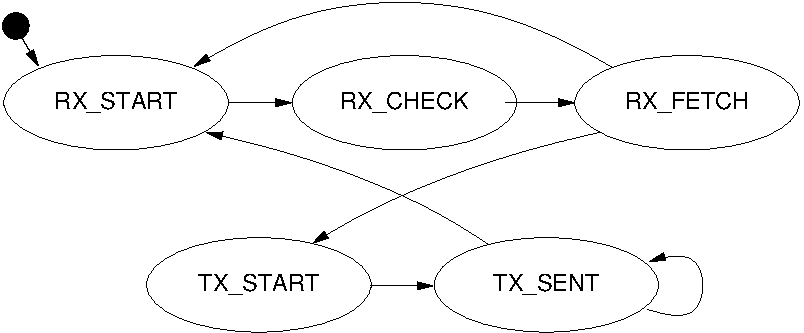
\includegraphics[width=.7\textwidth]{images/fsm-eoe} % FIXME
  \caption{Transition Diagram of the EoE State Machine}
  \label{fig:fsm-eoe}
\end{figure}

% FIXME

\begin{description}
\item[RX\_START] The beginning state of the EoE state machine. A
  mailbox check datagram is sent, to query the slave's mailbox for new
  frames. $\rightarrow$~RX\_CHECK

\item[RX\_CHECK] The mailbox check datagram is received. If the
  slave's mailbox did not contain data, a transmit cycle is started.
  $\rightarrow$~TX\_START

  If there are new data in the mailbox, a datagram is sent to fetch
  the new data. $\rightarrow$~RX\_FETCH

\item[RX\_FETCH] The fetch datagram is received. If the mailbox data
  do not contain a ``EoE Fragment request'' command, the data are
  dropped and a transmit sequence is started.
  $\rightarrow$~TX\_START

  If the received Ethernet frame fragment is the first fragment, a new
  socket buffer is allocated. In either case, the data are copied into
  the correct position of the socket buffer.

  If the fragment is the last fragment, the socket buffer is forwarded
  to the network stack and a transmit sequence is started.
  $\rightarrow$~TX\_START

  Otherwise, a new receive sequence is started to fetch the next
  fragment. $\rightarrow$~RX\_\-START

\item[TX\_START] The beginning state of a transmit sequence. It is
  checked, if the transmission queue contains a frame to send. If not,
  a receive sequence is started. $\rightarrow$~RX\_START

  If there is a frame to send, it is dequeued. If the queue was
  inactive before (because it was full), the queue is woken up with a
  call to \textit{netif\_wake\_queue()}. The first fragment of the
  frame is sent. $\rightarrow$~TX\_SENT

\item[TX\_SENT] It is checked, if the first fragment was sent
  successfully. If the current frame consists of further fragments,
  the next one is sent. $\rightarrow$~TX\_SENT

  If the last fragment was sent, a new receive sequence is started.
  $\rightarrow$~RX\_START
\end{description}

\paragraph{EoE Processing}

To execute the EoE state machine of every active EoE handler, there must be a
cyclic process. The easiest solution would be to execute the EoE state
machines synchronously with the master state machine (see
sec.~\ref{sec:fsm-master}). This approach has the following disadvantage:

Only one EoE fragment could be sent or received every few cycles. This
causes the data rate to be very low, because the EoE state machines are not
executed in the time between the application cycles. Moreover, the data rate
would be dependent on the period of the application task.

To overcome this problem, an own cyclic process is needed to asynchronously
execute the EoE state machines. For that, the master owns a kernel timer, that
is executed each timer interrupt. This guarantees a constant bandwidth, but
poses the new problem of concurrent access to the master. The locking
mechanisms needed for this are introduced in sec.~\ref{sec:concurr}.

\paragraph{Automatic Configuration}

By default, slaves are left in PREOP state, if no configuration is applied. If
an EoE interface link is set to ``up'', the requested slave's
application-layer state is automatically set to OP.

%------------------------------------------------------------------------------

\section{CANopen over EtherCAT (CoE)}
\label{sec:coe}
\index{CoE}

The CANopen over EtherCAT\nomenclature{CoE}{CANopen over EtherCAT, Mailbox
Protocol} protocol~\cite[sec.~5.6]{alspec} is used to configure slaves and
exchange data objects on application level.

% TODO
%
% Download / Upload
% Expedited / Normal
% Segmenting
% SDO Info Services
%

\paragraph{SDO Download State Machine}

The best time to apply SDO configurations is during the slave's PREOP state,
because mailbox communication is already possible and slave's application will
start with updating input data in the succeeding SAFEOP state. Therefore the
SDO configuration has to be part of the slave configuration state machine (see
sec.~\ref{sec:fsm-conf}): It is implemented via an SDO download state machine,
that is executed just before entering the slave's SAFEOP state. In this way,
it is guaranteed that the SDO configurations are applied each time, the slave
is reconfigured.

The transition diagram of the SDO Download state machine can be seen
in figure~\ref{fig:fsm-coedown}.

\begin{figure}[htbp]
  \centering
  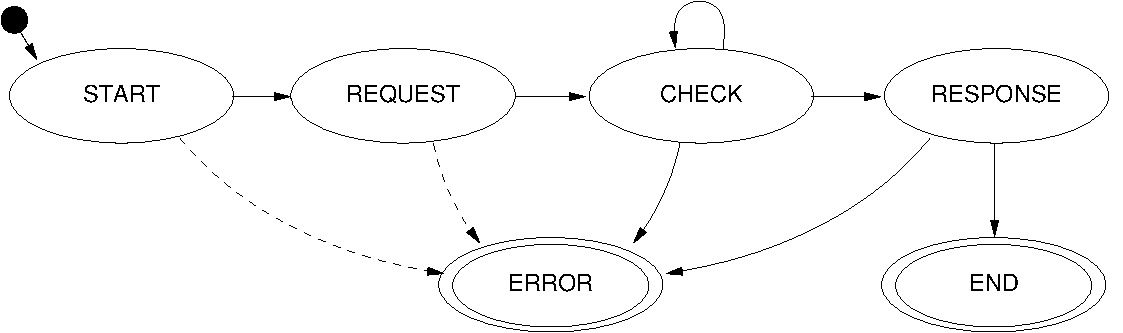
\includegraphics[width=.9\textwidth]{images/fsm-coedown} % FIXME
  \caption{Transition diagram of the CoE download state machine}
  \label{fig:fsm-coedown}
\end{figure}

% FIXME

\begin{description}
\item[START] The beginning state of the CoE download state
  machine. The ``SDO Download Normal Request'' mailbox command is
  sent. $\rightarrow$~REQUEST

\item[REQUEST] It is checked, if the CoE download request has been
  received by the slave. After that, a mailbox check command is issued
  and a timer is started. $\rightarrow$~CHECK

\item[CHECK] If no mailbox data is available, the timer is checked.
  \begin{itemize}
  \item If it timed out, the SDO download is aborted.
    $\rightarrow$~ERROR
  \item Otherwise, the mailbox is queried again.
    $\rightarrow$~CHECK
  \end{itemize}

  If the mailbox contains new data, the response is fetched.
  $\rightarrow$~RESPONSE

\item[RESPONSE] If the mailbox response could not be fetched, the data
  is invalid, the wrong protocol was received, or a ``Abort SDO
  Transfer Request'' was received, the SDO download is aborted.
  $\rightarrow$~ERROR

  If a ``SDO Download Normal Response'' acknowledgement was received,
  the SDO download was successful. $\rightarrow$~END

\item[END] The SDO download was successful.

\item[ERROR] The SDO download was aborted due to an error.

\end{description}

%------------------------------------------------------------------------------

\section{Vendor specific over EtherCAT (VoE)}
\label{sec:voe}
\index{VoE}

The VoE protocol opens the possibility to implement a vendor-specific mailbox
communication protocol. VoE mailbox messages are prepended by a VoE header
containing a 32-bit vendor ID and a 16-bit vendor-type. There are no more
constraints regarding this protocol.

The EtherCAT master allows to create multiple VoE handlers per slave
configuration via the application interface (see chap.~\ref{chap:api}). These
handlers contain the state machine necessary for the communication via VoE.

For more information about using VoE handlers, see sec.~\ref{sec:api-voe} or
the example applications provided in the \textit{examples/} subdirectory.

%------------------------------------------------------------------------------

\section{Servo Profile over EtherCAT (SoE)}
\label{sec:soe}
\index{SoE}

The SoE protocol implements the Service Channel layer, specified in IEC
61800-7 \cite{soespec} via EtherCAT mailboxes.

The SoE protocol is quite similar to the CoE protocol (see
sec.~\ref{sec:coe}). Instead of SDO indices and subindices, so-called
identification numbers (IDNs) identify parameters.

The implementation covers the ``SCC Read'' and ``SCC Write'' primitives, each
with the ability to fragment data.

There are several ways to use the SoE implementation:

\begin{itemize}

\item Reading and writing IDNs via the command-line tool (see
sec.~\ref{sec:soeaccess}).

\item Storing configurations for arbitrary IDNs via the application interface
(see chap.~\ref{chap:api}, i.\,e.~\lstinline+ecrt_slave_config_idn()+). These
configurations are written to the slave during configuration in PREOP state,
before going to SAFEOP.

\item The user-space library (see sec.~\ref{sec:userlib}), offers functions to
read/write IDNs in blocking mode (\lstinline+ecrt_master_read_idn()+,
\lstinline+ecrt_master_write_idn()+).

\end{itemize}

%------------------------------------------------------------------------------

\chapter{Userspace Interfaces}
\label{sec:user}
\index{Userspace}

For the master runs as a kernel module, accessing it is natively limited to
analyzing Syslog messages and controlling using \textit{modutils}.

It was necessary to implement further interfaces, that make it easier to access
the master from userspace and allow a finer influence. It should be possible
to view and to change special parameters at runtime.

Bus visualization is another point: For development and debugging purposes it
is necessary to show the connected slaves with a single command, for instance
(see sec.~\ref{sec:tool}).

The application interface has to be available in userspace, to allow userspace
programs to use EtherCAT master functionality. This was implemented via a
character device and a userspace library (see sec.~\ref{sec:userlib}).

Another aspect is automatic startup and configuration. The master must be able
to automatically start up with a persistent configuration (see
sec.~\ref{sec:system}).

A last thing is monitoring EtherCAT communication. For debugging purposes,
there had to be a way to analyze EtherCAT datagrams. The best way would be
with a popular network analyzer, like Wireshark \cite{wireshark} (the former
Ethereal) or others (see sec.~\ref{sec:debug}).

This chapter covers all these points and introduces the interfaces and tools
to make all that possible.

%------------------------------------------------------------------------------

\section{Command-line Tool}
\label{sec:tool}

% TODO --master

\subsection{Character Devices}
\label{sec:cdev}

Each master instance will get a character device as a userspace interface.
The devices are named \textit{/dev/EtherCATx}, where $x \in \{0 \ldots n\}$ is
the index of the master.

\paragraph{Device Node Creation} The character device nodes are automatically
created, if the \lstinline+udev+ Package is installed. See
sec.~\ref{sec:autonode} for how to install and configure it.

%------------------------------------------------------------------------------

\subsection{Setting Alias Addresses}
\label{sec:ethercat-alias}

\lstinputlisting[basicstyle=\ttfamily\footnotesize]{external/ethercat_alias}

%------------------------------------------------------------------------------

\subsection{Displaying the Bus Configuration}
\label{sec:ethercat-config}

\lstinputlisting[basicstyle=\ttfamily\footnotesize]{external/ethercat_config}

%------------------------------------------------------------------------------

\subsection{Output PDO information in C Language}
\label{sec:ethercat-cstruct}

\lstinputlisting[basicstyle=\ttfamily\footnotesize]{external/ethercat_cstruct}

%------------------------------------------------------------------------------

\subsection{Displaying Process Data}

\lstinputlisting[basicstyle=\ttfamily\footnotesize]{external/ethercat_data}

%------------------------------------------------------------------------------

\subsection{Setting a Master's Debug Level}
\label{sec:ethercat-debug}

\lstinputlisting[basicstyle=\ttfamily\footnotesize]{external/ethercat_debug}

%------------------------------------------------------------------------------

\subsection{Configured Domains}

\lstinputlisting[basicstyle=\ttfamily\footnotesize]{external/ethercat_domains}

%------------------------------------------------------------------------------

\subsection{SDO Access}

\lstinputlisting[basicstyle=\ttfamily\footnotesize]{external/ethercat_download}

\lstinputlisting[basicstyle=\ttfamily\footnotesize]{external/ethercat_upload}

%------------------------------------------------------------------------------

\subsection{EoE Statistics}

\lstinputlisting[basicstyle=\ttfamily\footnotesize]{external/ethercat_eoe}

%------------------------------------------------------------------------------

\subsection{File-Access over EtherCAT}

\lstinputlisting[basicstyle=\ttfamily\footnotesize]{external/ethercat_foe_read}

\lstinputlisting[basicstyle=\ttfamily\footnotesize]{external/ethercat_foe_write}

%------------------------------------------------------------------------------

\subsection{Creating Topology Graphs}

\lstinputlisting[basicstyle=\ttfamily\footnotesize]{external/ethercat_graph}

%------------------------------------------------------------------------------

\subsection{Master and Ethernet Devices}

\lstinputlisting[basicstyle=\ttfamily\footnotesize]{external/ethercat_master}

%------------------------------------------------------------------------------

\subsection{Sync Managers, PDOs and PDO Entries}

\lstinputlisting[basicstyle=\ttfamily\footnotesize]{external/ethercat_pdos}

%------------------------------------------------------------------------------

\subsection{Register Access}
\label{sec:regaccess}

\lstinputlisting[basicstyle=\ttfamily\footnotesize]{external/ethercat_reg_read}

\lstinputlisting[basicstyle=\ttfamily\footnotesize]{external/ethercat_reg_write}

%------------------------------------------------------------------------------

\subsection{SDO Dictionary}

\lstinputlisting[basicstyle=\ttfamily\footnotesize]{external/ethercat_sdos}

%------------------------------------------------------------------------------

\subsection{SII Access}
\label{sec:siiaccess}
\index{SII!Access}

It is possible to directly read or write the complete SII contents of the
slaves. This was introduced for the reasons below:

\begin{itemize}

\item The format of the SII data is still in development and categories can be
added in the future. With read and write access, the complete memory contents
can be easily backed up and restored.

\item Some SII data fields have to be altered (like the alias address). A quick
writing must be possible for that.

\item Through reading access, analyzing category data is possible from
userspace.

\end{itemize}

\lstinputlisting[basicstyle=\ttfamily\footnotesize]{external/ethercat_sii_read}

Reading out SII data is as easy as other commands. Though the data are in
binary format, analysis is easier with a tool like \textit{hexdump}:

\begin{lstlisting}
$ `\textbf{ethercat sii\_read --position 3 | hexdump}`
0000000 0103 0000 0000 0000 0000 0000 0000 008c
0000010 0002 0000 3052 07f0 0000 0000 0000 0000
0000020 0000 0000 0000 0000 0000 0000 0000 0000
...
\end{lstlisting}

Backing up SII contents can easily done with a redirection:

\begin{lstlisting}
$ `\textbf{ethercat sii\_read --position 3 > sii-of-slave3.bin}`
\end{lstlisting}

To download SII contents to a slave, writing access to the master's character
device is necessary (see sec.~\ref{sec:cdev}).

\lstinputlisting[basicstyle=\ttfamily\footnotesize]{external/ethercat_sii_write}

\begin{lstlisting}
# `\textbf{ethercat sii\_write --position 3 sii-of-slave3.bin}`
\end{lstlisting}

The SII contents will be checked for validity and then sent to the slave. The
write operation may take a few seconds.

%------------------------------------------------------------------------------

\subsection{Slaves on the Bus}

Slave information can be gathered with the subcommand \lstinline+slaves+:

\lstinputlisting[basicstyle=\ttfamily\footnotesize]{external/ethercat_slaves}

Below is a typical output:

\begin{lstlisting}
$ `\textbf{ethercat slaves}`
0     0:0  PREOP  +  EK1100 Ethernet Kopplerklemme (2A E-Bus)
1  5555:0  PREOP  +  EL3162 2K. Ana. Eingang 0-10V
2  5555:1  PREOP  +  EL4102 2K. Ana. Ausgang 0-10V
3  5555:2  PREOP  +  EL2004 4K. Dig. Ausgang 24V, 0,5A
\end{lstlisting}

%------------------------------------------------------------------------------

\subsection{SoE IDN Access}
\label{sec:soeaccess}

\lstinputlisting[basicstyle=\ttfamily\footnotesize]{external/ethercat_soe_read}

\lstinputlisting[basicstyle=\ttfamily\footnotesize]{external/ethercat_soe_write}

%------------------------------------------------------------------------------

\subsection{Requesting Application-Layer States}

\lstinputlisting[basicstyle=\ttfamily\footnotesize]{external/ethercat_states}

%------------------------------------------------------------------------------

\subsection{Displaying the Master Version}

\lstinputlisting[basicstyle=\ttfamily\footnotesize]{external/ethercat_version}

%------------------------------------------------------------------------------

\subsection{Generating Slave Description XML}

\lstinputlisting[basicstyle=\ttfamily\footnotesize]{external/ethercat_xml}

%------------------------------------------------------------------------------

\section{Userspace Library}
\label{sec:userlib}

The native application interface (see chap.~\ref{chap:api}) resides in
kernelspace and hence is only accessible from inside the kernel. To make the
application interface available from userspace programs, a userspace library
has been created, that can be linked to programs under the terms and
conditions of the LGPL, version 2 \cite{lgpl}.

The library is named \textit{libethercat}. Its sources reside in the
\textit{lib/} subdirectory and are build by default when using
\lstinline+make+. It is installed in the \textit{lib/} path below the
installation prefix as \textit{libethercat.a} (for static linking),
\textit{libethercat.la} (for the use with \textit{libtool}) and
\textit{libethercat.so} (for dynamic linking).

\subsection{Using the Library}

The application interface header \textit{ecrt.h} can be used both in kernel
and in user context.

The following minimal example shows how to build a program with EtherCAT
functionality. An entire example can be found in the \textit{examples/user/}
path of the master sources.

\begin{lstlisting}[language=C]
#include <ecrt.h>

int main(void)
{
    ec_master_t *master = ecrt_request_master(0);

    if (!master)
        return 1; // error

    pause(); // wait for signal
    return 0;
}
\end{lstlisting}

The program can be compiled and dynamically linked to the library with the
below command:

\begin{lstlisting}
gcc ethercat.c -o ectest -I/opt/etherlab/include \
    -L/opt/etherlab/lib -lethercat \
    -Wl,--rpath -Wl,/opt/etherlab/lib
\end{lstlisting}

The library can also be linked statically to the program:

\begin{lstlisting}
gcc -static ectest.c -o ectest -I/opt/etherlab/include \
    /opt/etherlab/lib/libethercat.a
\end{lstlisting}

\subsection{Implementation}
\label{sec:userimp}

Basically the kernel API was transferred into userspace via the master
character device (see chap.~\ref{chap:arch}, fig.~\ref{fig:arch} and
sec.~\ref{sec:cdev}).

The function calls of the kernel API are mapped to the userspace via an
\lstinline+ioctl()+ interface. The userspace API functions share a set of
generic \lstinline+ioctl()+ calls. The kernel part of the interface calls the
according API functions directly, what results in a minimum additional delay
(see sec.~\ref{sec:usertiming}).

For performance reasons, the actual domain process data (see
sec.~\ref{sec:processdata}) are not copied between kernel and user memory on
every access: Instead, the data are memory-mapped to the userspace
application. Once the master is configured and activated, the master module
creates one process data memory area spanning all domains and maps it to
userspace, so that the application can directly access the process data. As a
result, there is no additional delay when accessing process data from
userspace.

\paragraph{Kernel/User API Differences} Because of the memory-mapping of the
process data, the memory is managed internally by the library functions. As a
result, it is not possible to provide external memory for domains, like in the
kernel API. The corresponding functions are only available in kernelspace.
This is the only difference when using the application interface in userspace.

\subsection{Timing}
\label{sec:usertiming}

An interesting aspect is the timing of the userspace library calls compared to
those of the kernel API. Table~\ref{tab:usertiming} shows the call times and
standard deviancies of typical (and time-critical) API functions measured on
an Intel Pentium 4 M CPU with \unit{2.2}{\giga\hertz} and a standard 2.6.26
kernel.

\begin{table}[htbp]
  \centering
  \caption{Application Interface Timing Comparison}
  \label{tab:usertiming}
  \vspace{2mm}
  \begin{tabular}{l|c|c|c|c}

    &
    \multicolumn{2}{|c}{\textbf{Kernelspace}} &
    \multicolumn{2}{|c}{\textbf{Userspace}}  \\

    \textbf{Function} &
    $\mu(t)$ &
    $\sigma(t)$ &
    $\mu(t)$ &
    $\sigma(t)$ \\
    \hline

    \lstinline+ecrt_master_receive()+ &
    \unit{1.1}{\micro\second} &
    \unit{0.3}{\micro\second} &
    \unit{2.2}{\micro\second} &
    \unit{0.5}{\micro\second} \\

    \lstinline+ecrt_domain_process()+ &
    \unit{<0.1}{\micro\second} &
    \unit{<0.1}{\micro\second} &
    \unit{1.0}{\micro\second} &
    \unit{0.2}{\micro\second} \\

    \lstinline+ecrt_domain_queue()+ &
    \unit{<0.1}{\micro\second} &
    \unit{<0.1}{\micro\second} &
    \unit{1.0}{\micro\second} &
    \unit{0.1}{\micro\second} \\

    \lstinline+ecrt_master_send()+ &
    \unit{1.8}{\micro\second} &
    \unit{0.2}{\micro\second} &
    \unit{2.5}{\micro\second} &
    \unit{0.5}{\micro\second} \\

  \end{tabular}
\end{table}

The test results show, that for this configuration, the userspace API causes
about \unit{1}{\micro\second} additional delay for each function, compared to
the kernel API.

%------------------------------------------------------------------------------

\section{System Integration}
\label{sec:system}

To integrate the EtherCAT master as a service into a running system, it comes
with an init script and a sysconfig file, that are described below.

\subsection{Init Script}
\label{sec:init}
\index{Init script}

The EtherCAT master init script conforms to the requirements of the ``Linux
Standard Base'' (LSB\index{LSB}, \cite{lsb}). The script is installed to
\textit{etc/init.d/ethercat} below the installation prefix and has to be
copied (or better: linked) to the appropriate location (see
sec.~\ref{sec:installation}), before the master can be inserted as a service.
Please note, that the init script depends on the sysconfig file described
below.

To provide service dependencies (i.\,e.\ which services have to be started
before others) inside the init script code, LSB defines a special comment
block. System tools can extract this information to insert the EtherCAT init
script at the correct place in the startup sequence:

\lstinputlisting[firstline=38,lastline=48]
    {../script/init.d/ethercat}

\subsection{Sysconfig File}
\label{sec:sysconfig}
\index{Sysconfig file}

For persistent configuration, the init script uses a sysconfig file installed
to \textit{etc/sysconfig/ethercat} (below the installation prefix), that is
mandatory for the init script. The sysconfig file contains all configuration
variables needed to operate one or more masters. The documentation is inside
the file and included below:

\lstinputlisting[numbers=left,firstline=9,basicstyle=\ttfamily\scriptsize]
    {../script/sysconfig/ethercat}

\subsection{Starting the Master as a Service}
\label{sec:service}
\index{Service}

After the init script and the sysconfig file are placed into the right
location, the EtherCAT master can be inserted as a service. The different Linux
distributions offer different ways to mark a service for starting and stopping
in certain runlevels. For example, SUSE Linux provides the \textit{insserv}
command:

\begin{lstlisting}
# `\textbf{insserv ethercat}`
\end{lstlisting}

The init script can also be used for manually starting and stopping
the EtherCAT master. It has to be executed with one of the parameters
\texttt{start}, \texttt{stop}, \texttt{restart} or \texttt{status}.

\begin{lstlisting}[gobble=2]
  # `\textbf{/etc/init.d/ethercat restart}`
  Shutting down EtherCAT master                done
  Starting EtherCAT master                     done
\end{lstlisting}

%------------------------------------------------------------------------------

\section{Debug Interfaces}
\label{sec:debug}
\index{Debug Interfaces}

EtherCAT buses can always be monitored by inserting a switch between master
and slaves. This allows to connect another PC with a network monitor like
Wireshark~\cite{wireshark}, for example. It is also possible to listen to
local network interfaces on the machine running the EtherCAT master directly.
If the generic Ethernet driver (see sec.~\ref{sec:generic-driver}) is used,
the network monitor can directly listen on the network interface connected to
the EtherCAT bus.

When using native Ethernet drivers (see sec.~\ref{sec:native-drivers}), there
are no local network interfaces to listen to, because the Ethernet devices
used for EtherCAT are not registered at the network stack. For that case,
so-called ``debug interfaces'' are supported, which are virtual network
interfaces allowing to capture EtherCAT traffic with a network monitor (like
Wireshark or tcpdump) running on the master machine without using external
hardware. To use this functionality, the master sources have to be configured
with the \lstinline+--enable-debug-if+ switch (see
sec.~\ref{sec:installation}).

Every EtherCAT master registers a read-only network interface per attached
physical Ethernet device. The network interfaces are named \textit{ecdbgmX}
for the main device, and \textit{ecdbgbX} for the backup device (for future
use), where X is the master index. The below listing shows a debug interface
among some standard network interfaces:

\begin{lstlisting}
# `\textbf{ip link}`
1: lo: <LOOPBACK,UP> mtu 16436 qdisc noqueue
    link/loopback 00:00:00:00:00:00 brd 00:00:00:00:00:00
4: eth0: <BROADCAST,MULTICAST> mtu 1500 qdisc noop qlen 1000
    link/ether 00:13:46:3b:ad:d7 brd ff:ff:ff:ff:ff:ff
8: ecdbgm0: <BROADCAST,MULTICAST> mtu 1500 qdisc pfifo_fast
                                                 qlen 1000
    link/ether 00:04:61:03:d1:01 brd ff:ff:ff:ff:ff:ff
\end{lstlisting}

While a debug interface is enabled, all frames sent or received to or from the
physical device are additionally forwarded to the debug interface by the
corresponding master. Network interfaces can be enabled with the below
command:

\begin{lstlisting}
# `\textbf{ip link set dev ecdbgm0 up}`
\end{lstlisting}

Please note, that the frame rate can be very high. With an application
connected, the debug interface can produce thousands of frames per second.

\paragraph{Attention} The socket buffers needed for the operation of debug
interfaces have to be allocated dynamically. Some Linux realtime extensions
(like RTAI) do not allow this in realtime context!

%------------------------------------------------------------------------------

\chapter{Timing Aspects}
\label{sec:timing}

Although EtherCAT's timing is highly deterministic and therefore timing issues
are rare, there are a few aspects that can (and should be) dealt with.

%------------------------------------------------------------------------------

\subsection{Application Interface Profiling}
\label{sec:timing-profile}
\index{Profiling}
% FIXME

One of the most important timing aspects are the execution times of the
application interface functions, that are called in cyclic context. These
functions make up an important part of the overall timing of the application.
To measure the timing of the functions, the following code was used:

\begin{lstlisting}[gobble=2,language=C]
  c0 = get_cycles();
  ecrt_master_receive(master);
  c1 = get_cycles();
  ecrt_domain_process(domain1);
  c2 = get_cycles();
  ecrt_master_run(master);
  c3 = get_cycles();
  ecrt_master_send(master);
  c4 = get_cycles();
\end{lstlisting}

Between each call of an interface function, the CPU timestamp counter is read.
The counter differences are converted to \micro\second\ with help of the
\lstinline+cpu_khz+ variable, that contains the number of increments per
\milli\second.

For the actual measuring, a system with a \unit{2.0}{\giga\hertz} CPU was used,
that ran the above code in an RTAI thread with a period of
\unit{100}{\micro\second}. The measuring was repeated $n = 100$ times and the
results were averaged. These can be seen in table~\ref{tab:profile}.

\begin{table}[htpb]
  \centering
  \caption{Profiling of an Application Cycle on a \unit{2.0}{\giga\hertz}
  Processor}
  \label{tab:profile}
  \vspace{2mm}
  \begin{tabular}{l|r|r}
    Element & Mean Duration [\second] & Standard Deviancy [\micro\second] \\
    \hline
    \textit{ecrt\_master\_receive()} & 8.04 & 0.48\\
    \textit{ecrt\_domain\_process()} & 0.14 & 0.03\\
    \textit{ecrt\_master\_run()} & 0.29 & 0.12\\
    \textit{ecrt\_master\_send()} & 2.18 & 0.17\\ \hline
    Complete Cycle & 10.65 & 0.69\\ \hline
  \end{tabular}
\end{table}

It is obvious, that the functions accessing hardware make up the
lion's share. The \textit{ec\_master\_receive()} executes the ISR of
the Ethernet device, analyzes datagrams and copies their contents into
the memory of the datagram objects. The \textit{ec\_master\_send()}
assembles a frame out of different datagrams and copies it to the
hardware buffers. Interestingly, this makes up only a quarter of the
receiving time.

The functions that only operate on the masters internal data structures are
very fast ($\Delta t < \unit{1}{\micro\second}$). Interestingly the runtime of
\textit{ec\_domain\_process()} has a small standard deviancy relative to the
mean value, while this ratio is about twice as big for
\textit{ec\_master\_run()}: This probably results from the latter function
having to execute code depending on the current state and the different state
functions are more or less complex.

For a realtime cycle makes up about \unit{10}{\micro\second}, the theoretical
frequency can be up to \unit{100}{\kilo\hertz}. For two reasons, this frequency
keeps being theoretical:

\begin{enumerate}

\item The processor must still be able to run the operating system between the
realtime cycles.

\item The EtherCAT frame must be sent and received, before the next realtime
cycle begins. The determination of the bus cycle time is difficult and covered
in sec.~\ref{sec:timing-bus}.

\end{enumerate}

%------------------------------------------------------------------------------

\subsection{Bus Cycle Measuring}
\label{sec:timing-bus}
\index{Bus cycle}

For measuring the time, a frame is ``on the wire'', two timestamps must be
taken:

\begin{enumerate}

\item The time, the Ethernet hardware begins with physically sending the
frame.

\item The time, the frame is completely received by the Ethernet hardware.

\end{enumerate}

Both times are difficult to determine. The first reason is, that the
interrupts are disabled and the master is not notified, when a frame is sent
or received (polling would distort the results). The second reason is, that
even with interrupts enabled, the time from the event to the notification is
unknown. Therefore the only way to confidently determine the bus cycle time is
an electrical measuring.

Anyway, the bus cycle time is an important factor when designing realtime
code, because it limits the maximum frequency for the cyclic task of the
application.  In practice, these timing parameters are highly dependent on the
hardware and often a trial and error method must be used to determine the
limits of the system.

The central question is: What happens, if the cycle frequency is too high? The
answer is, that the EtherCAT frames that have been sent at the end of the
cycle are not yet received, when the next cycle starts.  First this is noticed
by \textit{ecrt\_domain\_process()}, because the working counter of the
process data datagrams were not increased. The function will notify the user
via Syslog\footnote{To limit Syslog output, a mechanism has been implemented,
that outputs a summarized notification at maximum once a second.}. In this
case, the process data keeps being the same as in the last cycle, because it
is not erased by the domain. When the domain datagrams are queued again, the
master notices, that they are already queued (and marked as sent). The master
will mark them as unsent again and output a warning, that datagrams were
``skipped''.

On the mentioned \unit{2.0}{\giga\hertz} system, the possible cycle frequency
can be up to \unit{25}{\kilo\hertz} without skipped frames. This value can
surely be increased by choosing faster hardware. Especially the RealTek
network hardware could be replaced by a faster one. Besides, implementing a
dedicated ISR for EtherCAT devices would also contribute to increasing the
latency. These are two points on the author's to-do list.

%------------------------------------------------------------------------------

\chapter{Installation}
\label{sec:installation}
\index{Master!Installation}

\section{Getting the Software}
\label{sec:getting}

There are several ways to get the master software:

\begin{enumerate}

\item An official release (for example \masterversion), can be downloaded from
the master's website\footnote{\url{http://etherlab.org/en/ethercat/index.php}}
at~the EtherLab project~\cite{etherlab} as a tarball.

\item The most recent development revision (and moreover any other revision)
can be obtained via the Mercurial~\cite{mercurial} repository on the master's
project page on
SourceForge.net\footnote{\url{http://sourceforge.net/projects/etherlabmaster}}.
The whole repository can be cloned with the command

\begin{lstlisting}[breaklines=true]
hg clone http://etherlabmaster.hg.sourceforge.net/hgweb/etherlabmaster/etherlabmaster `\textit{local-dir}`
\end{lstlisting}

\item Without a local Mercurial installation, tarballs of arbitrary revisions
can be downloaded via the ``bz2'' links in the browsable repository
pages\footnote{\url{http://etherlabmaster.hg.sourceforge.net/hgweb/etherlabmaster/etherlabmaster}}.

\end{enumerate}

\section{Building the Software}

After downloading a tarball or cloning the repository as described in
sec.~\ref{sec:getting}, the sources have to be prepared and configured for the
build process.

When a tarball was downloaded, it has to be extracted with the following
commands:

\begin{lstlisting}[gobble=2]
  $ `\textbf{tar xjf ethercat-\masterversion.tar.bz2}`
  $ `\textbf{cd ethercat-\masterversion/}`
\end{lstlisting}

The software configuration is managed with Autoconf~\cite{autoconf} so the
released versions contain a \lstinline+configure+ shell script, that has to be
executed for configuration (see below).

\paragraph{Bootstrap} When downloading or cloning directly from the
repository, the \lstinline+configure+ script does not yet exist. It can be
created via the \lstinline+bootstrap.sh+ script in the master sources. The
autoconf and automake packages are required for this.

\paragraph{Configuration and Build} The configuration and the build process
follow the below commands:

\begin{lstlisting}[gobble=2]
  $ `\textbf{./configure}`
  $ `\textbf{make}`
  $ `\textbf{make modules}`
\end{lstlisting}

Table~\ref{tab:config} lists important configuration switches and options.

\begin{table}
  \caption{Configuration options}
  \label{tab:config}
  \vspace{2mm}
  \begin{tabular}{l|p{.3\textwidth}|l}

\bf Option/Switch & \bf Description & \bf Default\\\hline

\lstinline+--prefix+ & Installation prefix & \textit{/opt/etherlab}\\

\lstinline+--with-linux-dir+ & Linux kernel sources & Use running kernel\\

\lstinline+--with-rtai-dir+ & RTAI path (only for RTAI example) & \\

\hline

\lstinline+--enable-tool+ & Build the command-line tool ``ethercat'' (see
sec.~\ref{sec:tool}). & yes\\

\lstinline+--enable-userlib+ & Build the userspace library. & yes\\

\lstinline+--enable-eoe+ & Enable EoE support & yes\\

\lstinline+--enable-cycles+ & Use CPU timestamp counter. Enable this on Intel
architecture to get finer timing calculation. & no\\

\lstinline+--enable-debug-if+ & Create a debug interface for each master & no\\

\lstinline+--enable-debug-ring+ & Create a debug ring to record frames & no\\

\hline

\lstinline+--enable-8139too+ & Build the 8139too driver & yes\\

\lstinline+--with-8139too-kernel+ & 8139too kernel & $\dagger$\\

\lstinline+--enable-e100+ & Build the e100 driver & no\\

\lstinline+--with-e100-kernel+ & e100 kernel & $\dagger$\\

\lstinline+--enable-e1000+ & Enable e1000 driver & no\\

\lstinline+--with-e1000-kernel+ & e1000 kernel & $\dagger$\\

\lstinline+--enable-e1000e+ & Enable e1000e driver & no\\

\lstinline+--with-e1000e-kernel+ & e1000e kernel & $\dagger$\\

\lstinline+--enable-r8169+ & Enable r8169 driver & no\\

\lstinline+--with-r8169-kernel+ & r8169 kernel & $\dagger$\\

\lstinline+--enable-generic+ & Build the generic Ethernet driver (see
sec.~\ref{sec:generic-driver}). & no\\

  \end{tabular}
  \vspace{2mm}

\begin{description}

\item[$\dagger$] If this option is not specified, the kernel version to use is
extracted from the Linux kernel sources.

\end{description}

\end{table}

\section{Building the Interface Documentation}
\label{sec:gendoc}

The source code is documented using Doxygen~\cite{doxygen}. To build the HTML
documentation, the Doxygen software has to be installed. The below command
will generate the documents in the subdirectory \textit{doxygen-output}:

\begin{lstlisting}
$ `\textbf{make doc}`
\end{lstlisting}

The interface documentation can be viewed by pointing a browser to the file
\textit{doxygen-output/html/index.html}. The functions and data structures of
the application interface a covered by an own module ``Application
Interface''.

\section{Installing the Software}

The below commands have to be entered as \textit{root}: The first one will
install the EtherCAT header, init script, sysconfig file and the userspace
tool to the prefix path. The second one will install the kernel modules to the
kernel's modules directory. The final \lstinline+depmod+ call is necessary to
include the kernel modules into the \textit{modules.dep} file to make it
available to the \lstinline+modprobe+ command, used in the init script. 

\begin{lstlisting}
# `\textbf{make install}`
# `\textbf{make modules\_install}`
# `\textbf{depmod}`
\end{lstlisting}

If the target kernel's modules directory is not under \textit{/lib/modules}, a
different destination directory can be specified with the \lstinline+DESTDIR+
make variable. For example:

\begin{lstlisting}
# `\textbf{make DESTDIR=/vol/nfs/root modules\_install}`
\end{lstlisting}

This command will install the compiled kernel modules to
\textit{/vol/nfs/root/lib/modules}, prepended by the kernel release.

If the EtherCAT master shall be run as a service\footnote{Even if the EtherCAT
master shall not be loaded on system startup, the use of the init script is
recommended for manual (un-)loading.} (see sec.~\ref{sec:system}), the init
script and the sysconfig file have to be copied (or linked) to the appropriate
locations. The below example is suitable for SUSE Linux. It may vary for other
distributions.

% FIXME relative ln -s?
\begin{lstlisting}
# `\textbf{cd /opt/etherlab}`
# `\textbf{cp etc/sysconfig/ethercat /etc/sysconfig/}`
# `\textbf{ln -s etc/init.d/ethercat /etc/init.d/}`
# `\textbf{insserv ethercat}`
\end{lstlisting}

Now the sysconfig file \texttt{/etc/sysconfig/ethercat} (see
sec.~\ref{sec:sysconfig}) has to be customized. The minimal customization is
to set the \lstinline+MASTER0_DEVICE+ variable to the MAC address of the
Ethernet device to use (or \lstinline+ff:ff:ff:ff:ff:ff+ to use the first
device offered) and selecting the driver(s) to load via the
\lstinline+DEVICE_MODULES+ variable.

After the basic configuration is done, the master can be started with the
below command:

\begin{lstlisting}
# `\textbf{/etc/init.d/ethercat start}`
\end{lstlisting}

At this time, the operation of the master can be observed by viewing the
Syslog\index{Syslog} messages, which should look like the ones below. If
EtherCAT slaves are connected to the master's EtherCAT device, the activity
indicators should begin to flash.

\begin{lstlisting}[numbers=left]
EtherCAT: Master driver `\masterversion`
EtherCAT: 1 master waiting for devices.
EtherCAT Intel(R) PRO/1000 Network Driver - version 6.0.60-k2
Copyright (c) 1999-2005 Intel Corporation.
PCI: Found IRQ 12 for device 0000:01:01.0
PCI: Sharing IRQ 12 with 0000:00:1d.2
PCI: Sharing IRQ 12 with 0000:00:1f.1
EtherCAT: Accepting device 00:0E:0C:DA:A2:20 for master 0.
EtherCAT: Starting master thread.
ec_e1000: ec0: e1000_probe: Intel(R) PRO/1000 Network
          Connection
ec_e1000: ec0: e1000_watchdog_task: NIC Link is Up 100 Mbps
          Full Duplex
EtherCAT: Link state changed to UP.
EtherCAT: 7 slave(s) responding.
EtherCAT: Slave states: PREOP.
EtherCAT: Scanning bus.
EtherCAT: Bus scanning completed in 431 ms.
\end{lstlisting}

\begin{description}

\item[\linenum{1} -- \linenum{2}] The master module is loading, and one master
is initialized.

\item[\linenum{3} -- \linenum{8}] The EtherCAT-capable e1000 driver is
loading. The master accepts the device with the address
\lstinline+00:0E:0C:DA:A2:20+.

\item[\linenum{9} -- \linenum{16}] The master goes to idle phase, starts its
state machine and begins scanning the bus.

\end{description}

\section{Automatic Device Node Creation}
\label{sec:autonode}

The \lstinline+ethercat+ command-line tool (see sec.~\ref{sec:tool})
communicates with the master via a character device. The corresponding device
nodes are created automatically, if the udev daemon is running.  Note, that on
some distributions, the \lstinline+udev+ package is not installed by default.

The device nodes will be created with mode \lstinline+0660+ and group
\lstinline+root+ by default. If ``normal'' users shall have reading access, a
udev rule file (for example \textit{/etc/udev/rules.d/99-EtherCAT.rules}) has
to be created with the following contents:

\begin{lstlisting}
KERNEL=="EtherCAT[0-9]*", MODE="0664"
\end{lstlisting}

After the udev rule file is created and the EtherCAT master is restarted with
\lstinline[breaklines=true]+/etc/init.d/ethercat restart+, the device node
will be automatically created with the desired rights:

\begin{lstlisting}
# `\textbf{ls -l /dev/EtherCAT0}`
crw-rw-r--  1 root root 252, 0 2008-09-03 16:19 /dev/EtherCAT0
\end{lstlisting}

Now, the \lstinline+ethercat+ tool can be used (see sec.~\ref{sec:tool}) even
as a non-root user.

If non-root users shall have writing access, the following udev rule can be
used instead:

\begin{lstlisting}
KERNEL=="EtherCAT[0-9]*", MODE="0664", GROUP="users"
\end{lstlisting}

%------------------------------------------------------------------------------

\begin{thebibliography}{99}

\bibitem{etherlab} Ingenieurgemeinschaft IgH: EtherLab -- Open Source Toolkit
for rapid realtime code generation under Linux with Simulink/RTW and EtherCAT
technology. \url{http://etherlab.org/en}, 2008.

\bibitem{dlspec} IEC 61158-4-12: Data-link Protocol Specification.
International Electrotechnical Commission (IEC), 2005.

\bibitem{alspec} IEC 61158-6-12: Application Layer Protocol Specification.
International Electrotechnical Commission (IEC), 2005.

\bibitem{gpl} GNU General Public License, Version 2.
\url{http://www.gnu.org/licenses/gpl-2.0.html}. October~15, 2008.

\bibitem{lgpl} GNU Lesser General Public License, Version 2.1.
\url{http://www.gnu.org/licenses/old-licenses/lgpl-2.1.html}. October~15,
2008.

\bibitem{lsb} Linux Standard Base.
\url{http://www.linuxfoundation.org/en/LSB}. August~9, 2006.

\bibitem{wireshark} Wireshark. \url{http://www.wireshark.org}. 2008.

\bibitem{automata} {\it Hopcroft, J.\,E.\ / Ullman, J.\,D.}: Introduction to
Automata Theory, Languages and Computation. Adison-Wesley, Reading,
Mass.~1979.

\bibitem{fsmmis} {\it Wagner, F.\ / Wolstenholme, P.}: State machine
misunderstandings. In: IEE journal ``Computing and Control Engineering'',
2004.

\bibitem{rtai} RTAI. The RealTime Application Interface for Linux from DIAPM.
\url{https://www.rtai.org}, 2010.

\bibitem{rt-preempt} RT PREEMPT HOWTO.
\url{http://rt.wiki.kernel.org/index.php/RT_PREEMPT_HOWTO}, 2010.

\bibitem{doxygen} Doxygen. Source code documentation generator tool.
\url{http://www.stack.nl/~dimitri/doxygen}, 2008.

\bibitem{mercurial} Mercurial SCM. \url{http://mercurial.selenic.com}, 2010.

\bibitem{autoconf} Autoconf -- GNU Project -- Free Software Foundation (FSF).
\url{http://www.gnu.org/software/autoconf}, 2010.

\bibitem{soespec} IEC 61800-7-304: Adjustable speed electrical power drive
systems - Part 7-300: Generic interface and use of profiles for power drive
systems - Mapping of profiles to network technologies. International
Electrotechnical Commission (IEC), 2007.

\end{thebibliography}

\printnomenclature
\addcontentsline{toc}{chapter}{\nomname}
\markleft{\nomname}

\printindex
\markleft{Index}

%------------------------------------------------------------------------------

\end{document}

%------------------------------------------------------------------------------
